% Yvonnick Esnault - yvonnick.e@free.fr 
% Gaetan Le Brun - gaetan.lebrun@gmail.com
% Thibaut Leli�vre - thibaut.lelievre@voila.fr
% Vincent Mah� - vmahe@free.fr
% Les chapitres peuvent commencer sur une page paire ou impaire
%openany
\documentclass[a4paper,11pt]{article}
%\frontmatter

\usepackage[T1]{fontenc}
\usepackage{ae,aecompl}
\usepackage[frenchb]{babel}
\usepackage[pdftex]{graphicx}
\usepackage[french]{minitoc}
\usepackage{fancyhdr}
\usepackage{lastpage}
\usepackage{hyperref}
\usepackage{textcomp}
%\usepackage [applemac] {inputenc} % les accents
\usepackage{verbatim}
\usepackage{float}

\evensidemargin=13pt
\oddsidemargin=13pt
\topmargin=-\headheight \advance\topmargin by -\headsep
\textwidth=14.59cm \textheight=21.62cm % normal A4, 1'' margin % 24.62cm
\setlength{\parindent}{8mm} % on remet le retrait de paragraphe

%%% My Vars %%%
\def\mytitle{TetraHead}
\def\mysubject{Synth\'etiseur}
\def\mydate{\today}
\def\myversion{1.0}
\def\me{\small  Yvonnick Esnault - Ga�tan Le Brun - Thibaut Leli�vre - Vincent Mah�}
\def\meandmail{\me \\{\normalsize\tt \mymail}}

%%% Fancy headers to add logo, line \ldots{} %%%
\pagestyle{fancy}
\fancyhf{}

% red�finition du style plain pour les pages sp�ciales (chapter)
\fancypagestyle{plain}{
 \fancyhead{}
 \renewcommand{\headrulewidth}{0pt}
 \renewcommand{\footrulewidth}{0.4pt}
 \lfoot{\textsl{\me\space} \\
\mysubject}
 \cfoot{}
 \rfoot{\textsl{Page \thepage \space sur \pageref{LastPage} }}
}

\renewcommand{\headsep}{50pt}

%\renewcommand{\chaptermark}[1]{\markboth{#1}{}}
\renewcommand{\sectionmark}[1]{\markright{#1}}
%\lhead[\thepage]{\rightmark}
%\rhead[\leftmark]{\thepage}

% Header
%\lhead{\includegraphics[width=2cm]{../document_type/images/logo.png}}
\chead{\mysubject} %\leftmark : contient le nom du chapitre courant.
%\rhead{\includegraphics[width=2cm]{images/logo_itin.png}}

%Footer
\lfoot{\textsl{\me\space}}
\cfoot{}
\rfoot{\textsl{Page \thepage \space sur \pageref{LastPage} }}

%Affiche les ligne en haut, et en bas
\renewcommand{\headrulewidth}{0.4pt}
\renewcommand{\footrulewidth}{0.4pt}

%%% bookmarks, linking in pdf %%%
\hypersetup{pdfauthor={\me},%
            pdftitle={\mytitle},%
            pdfsubject={\mysubject},%
            colorlinks,%
            citecolor=black,%
            filecolor=black,%
            linkcolor=black,%
            urlcolor=black,%
            pdftex}

%%% Commande pour supprimer en-t�tes
%%% et pied de page des pages vides
\newcommand{\clearemptydoublepage}{%
\newpage{\pagestyle{empty}\cleardoublepage}}

%%% Environnement pour le tableau de l'historique
\newenvironment{historique}
{

\begin{center}
{\huge \textbf{Historique}}

\vspace{3cm}
\begin{tabular}{|l|l|l|l|}
\hline
\textbf{Date} & \textbf{Auteur} & \textbf{Modifications} & \textbf{Version} \\
\hline
}
{
\end{tabular}\end{center}
\newpage
}

\newcommand{\histo}[4]
{#1 & #2 & #3 & #4 \\
\hline
}


%\newcommand{\info}[1]{
%\begin{figure}
%  \framebox[\textwidth][l]{
%   \begin{minipage}[c]{0.1\textwidth}
%     \medskip
%
%      
\includegraphics{../document_type/images/info.png}
%      \medskip
%
%   \end{minipage} \hfill
%   \begin{minipage}[c]{0.8\textwidth}
%     \medskip
%
%     #1\medskip
%
%   \end{minipage} \hfill
%   \begin{minipage}[c]{0.1\textwidth}
%     \makebox[30pt]{}\par
%   \end{minipage}
%}
%\end{figure}
%}

\newcommand{\encadre}[2]{
\begin{figure}[!h]
  \framebox[\textwidth][l]{
   \begin{minipage}[c]{0.1\textwidth}
     \medskip

      \includegraphics{#1}
      \medskip

   \end{minipage} \hfill
   \begin{minipage}[c]{0.8\textwidth}
     \medskip

     #2\medskip

   \end{minipage} \hfill
   \begin{minipage}[c]{0.1\textwidth}
     \makebox[30pt]{}\par
   \end{minipage}
}
\end{figure}
}

\newcommand{\info}[1]{
\encadre{../document_type/images/info.png}{#1}
}

\newcommand{\attention}[1]{
\encadre{../document_type/images/attention.png}{#1}
}

\newcommand{\code}[1]{\texttt{#1}}

\newcommand{\subsubsubsection}[1]{\textbf{#1}
\medskip

}

\usepackage{url}
\usepackage{makeidx}

% Titre du document qui apparait sur la premi�re page
\newcommand{\titre}{Dossier de conception (PSM)}


% Les param�tres suivants remplissent le tableau de propri�t�.
% Pour le param�tre \diffusion mettre en gras celui qui nous int�resse
\newcommand{\diffusion}{\textbf{Libre} & Restreint & Confidentiel}
\newcommand{\etat}{Applicable}
\newcommand{\version}{1.6}
\newcommand{\datedoc}{15/02/2006}
\makeindex

% D�but du document
\begin{document}

% Cr�e la premi�re page
%\pagenumbering{Arabic}

\newlength{\larg}
\setlength{\larg}{14.5cm}

\begin{titlepage}

\begin{center}

\includegraphics{../document_type/images/logo_TetraHead_small.png}\\
\end{center}
 
 %\vspace{5.5cm}
 \vspace{\stretch{1}}

{\rule{\larg}{1mm}}\vspace{7mm}
\begin{center}
  {\Huge {\bf {TetraHead - Synth\'etiseur}}} \\
  \medskip
  {\huge \titre}
\end{center}

\vspace{2mm}

{\rule{\larg}{1mm}}
\vspace{2mm} \\
\begin{tabular}{p{11cm} r}
   & {\large \bf 2006}% \\
%   & {\large  \today}
\end{tabular}\\
%\vspace{3cm}
\vspace{\stretch{1}}

\medskip

\begin{center}
\begin{tabular}{|l|l|l|l|}
\hline
\textbf{Diffusion} & \diffusion \\
\hline
�tat & \multicolumn{3}{|l|}{\textbf{\etat}} \\
\hline
Version & \multicolumn{3}{|l|}{\textbf{\version}} \\
\hline
Date & \multicolumn{3}{|l|}{\textbf{\datedoc}} \\
\hline
\end{tabular}

\end{center}

\end{titlepage}



% Historique du document. 
\begin{historique}
% Il faut ajouter une balise \histo pour chaque mise � jour
% du document.
% \histo{Date}{Pr�nom Nom}{Modification}{Version}
\histo{28/01/2006}{Yvonnick Esnault}{Cr�ation}{1.0}
\histo{08/02/2006}{Yvonnick Esnault}{Mise � jour}{1.1}
\histo{11/02/2006}{Vincent Mah�}{Moteur}{1.2}
\histo{10/02/2006}{Ga�tan Le Brun}{Mod�le PAC et digrammes UML}{1.3}
\histo{13/02/2006}{Thibaut Leli�vre}{Interface}{1.4}
\histo{14/02/2006}{Vincent Mah�}{Relecture}{1.5}
\histo{15/02/2006}{Thibaut Leli�vre}{Relecture}{1.6}
\end{historique}

\tableofcontents
\newpage

\listoffigures
\newpage

\section{Description}

Ce document d�crit les �l�ments de conception relatifs au projet, principalement
une description pr�cise des diff�rents modules, l'architecture de l'application (diagrammes UML).

Les sources sont divis�es en deux grands paquetages principaux, le \emph{core} 
et la \emph{GUI}, eux-m�mes subdivis�s en plusieurs paquetages adhoc.
\emph{Core} correspond au mod�le m�tier et \emph{GUI} � l'interface graphique qui permet 
d'agir sur le mod�le tout en restant totalement ind�pendant de l'impl�mentation, en se basant
sur le mod�le \emph{PAC}, section~\ref{pac}, page~\pageref{pac}.

\begin{figure}[!h]
	\begin{center} 
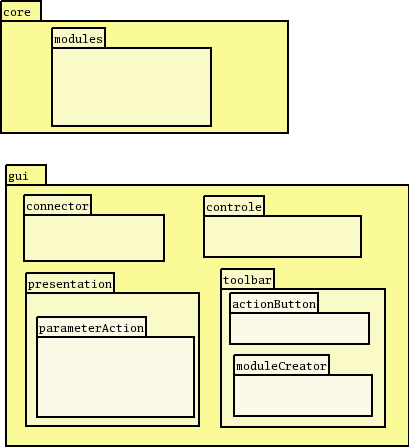
\includegraphics[scale=0.5]{img/paquetages.png}
		\caption{Diagramme des paquetages}
		\label{paquetages}
	\end{center}
\end{figure}

\section{Moteur de Son}
\label{moteur audio}
\subsection{Points Cl�s}
\begin{itemize}
  \item La communication entre les modules doit se faire valeur par valeur et 
  non par le biais d'un buffer,
  \item La valeur transmise est un flottant ayant une valeur entre -5 et +5, correspondant � la tension �lectrique utilis�e dans un synth�tiseur �lectronique r�el,
  \item La classe \code{Synthetizer} comporte un ensemble de modules et lorsqu'il est 
  en cours de jeu, il appelle la m�thode \code{compute()} sur tous les modules, 
  peu importe leur ordre.
\end{itemize}

\subsection{Synth�tiseur et s�quenceur}
Le r�le de l'objet \code{Synthetizer} est d'appeler la m�thode \code{compute()}
de chaque module qu'il poss�de, lorsque l'utilisateur le passe dans l'�tat \code{playing}.

Les principales m�thodes que l'on doit retrouver dans cet objet sont : 
\begin{itemize}
  \item \code{addModule(IModule)}
  \item \code{playSynthetizer()}
  \item \code{stopSynthetizer()}
\end{itemize}

Le Synthetizer g�re �galement la fr�quence d'�chantillonage\index{Frequence 
d'echantillonage@Fr�quence d'�chantillonage} par d�faut, que chaque module doit 
conna�tre.

Lorsque le synth�tiseur est en cours de marche, il ne doit pas bloquer l'interface
graphique. Il faut donc le lancer dans un \code{Thread} et d�finir une m�thode
\code{run()}. Cette m�thode contiendra le s�quenceur qui sera tel que : 

\begin{verbatim}
    TantQue etat == marche
      Pour Tous les modules m dans listeModules
        m.compute()
      FinPour  
    FinTantQue
\end{verbatim}

\subsubsection{Boucle dans le montage}
Le s�quenceur lance les m�thodes \code{compute()} de ses modules dans l'ordre o� ils ont
�t� rajout�s sur le montage. Il n'y a pas de gain visible � apporter un 
ordre dans les modules.
Cette m�thode permet d'effectuer des boucles dans le montage de mani�re
transparente, chaque module lisant la valeur de chaque port d'entr�e, traitant puis
�crivant la valeur sur le port de sortie. Si son port de sortie est connect� sur 
le port d'entr�e (ce qui est possible), il n'y a pas de probl�me a priori.

\subsection{Description des modules}
\index{Module!Description}
Tous les modules doivent �tendre une classe abstraite : \code{Module}. Cette 
classe impl�mente une interface \code{IModule}. Les d�tails des m�thodes et des 
attributs sont visibles dans les diagrammes UML de ce chapitre.

Globalement, cette classe poss�de un ensemble de ports d'entr�es, un port de 
sortie, un ensemble de param�tres discrets, un ensemble de param�tres continus. 
Chaque attribut peut �tre NULL.

Les ports d'entr�es ainsi que les param�tres discrets et continus sont g�r�s 
par le biais de collections \code{HashMap}, pour plus de performance et pour un 
acc�s direct (n�cessit� par certains algorithmes � chaque ex�cution de 
\code{compute}).

\subsubsection{LFO}
Un \emph{Low Frequency Oscillator} g�n�re une onde de basse fr�quence, pouvant 
�tre utilis�e comme param�tre d'entr�e dans d'autres modules.

Le signal carr� est g�n�ralement l'onde choisie pour d�clencher un top (dans 
l'ADSR Trigger par exemple).

R�sum� de la composition :
\begin{itemize}
\item Port(s) IN : NULL.
\item Port OUT : 1.
\item Param�tre(s) continu(s): pitch avec une plage de 0 � 20 Hz.
\item Param�tre(s) discret(s): Forme du signal g�n�r� : carr�, sinuso�dal, dent 
de scie (+ inverse), triangle.
\end{itemize}

\medskip

\subsubsubsection{Algorithmes}
\index{Algorithme!LFO}
Les diff�rents algorithmes n�cessaires � l'obtention des profils d'ondes 
demand�s ont �t� con�us ex nihilo par l'�quipe TetraHead en analysant 
math�matiquement le r�sultat souhait� pour les $n$ �chantillons d'une p�riode 
d'onde donn�e. la valeur $n~=~freqEch~/~pitch$ o� $freqEch$ d�signe la 
fr�quence d'�chantillonnage \index{Frequence d'echantillonage@Fr�quence 
d'�chantillonage}du signal (choisie au niveau du synth�tiseur) et $pitch$ la 
fr�quence d�sir�e pour le signal (440 Hz pour un \emph{LA}).
\begin{description}
\index{Onde}
 \item[Onde carr�e :] le signal vaut $+5$ (volts) pour $n/2$ valeurs puis $-5$ 
 pour $n/2$ valeurs.
 \item[Onde toit d'usine :] le signal part de $-5$ au d�but de la p�riode puis 
 cro�t de $10/n$ � chaque �chantillon, pour finir � $+5$ en fin de p�riode
 \item[Onde dents de scie :] le signal part de $+5$ au d�but de la p�riode puis 
 d�cro�t de $10/n$ � chaque �chantillon, pour finir � $-5$ en fin de p�riode
 \item[Onde triangulaire :] le signal part de $-5$ au d�but de la p�riode puis 
 cro�t de $5/n$ � chaque �chantillon, jusqu'� atteindre $+5$ au $n/2$ 
 �chantillon. Il d�cro�t ensuite au m�me rythme, pour finir � $-5$ en fin de 
 p�riode.
 \item[Onde sinuso�dale :] revient � calculer la hauteur atteinte par un rayon 
 de longueur $1$ sur un cercle en fonction d'un incr�ment de la valeur 
 horizontale allant de $-1$ � $+1$ pour un indice $i$ allant de $0$ � $n$. 
 La hauteur se calcule par la formule suivante : $5\cdot\sin(2\cdot i\cdot\pi/n))$.
\end{description} 

\subsubsection{VCO}
Un \emph{Voltage Controlled Oscillator} est similaire au LFO, mais avec un port 
d'entr�e Pitch-IN\index{Pitch-In} (pour brancher un LFO par exemple) et une 
plage de valeur de Pitch\index{Pitch} dans les fr�quences audibles.

R�sum� de la composition :
\begin{itemize}
\item Port(s) IN : 1 pitch-in.
\item Port OUT : 1.
\item Param�tre(s) continu(s): Pitch en hertz. Valeur minimum : 20 Hz. Valeur 
maximum : 3520 Hz.
\item Param�tre(s) discret(s): similaire au LFO.
\end{itemize}

\medskip

\subsubsubsection{Algorithmes}
\index{Algorithme!VCO}
Les algorithmes de calcul des ondes, dans le \code{LFO}, ont �t� s�par�s de la 
m�thode \code{compute()}, cette derni�re ne faisant plus que le calcul du 
nombre d'�chantillons par p�riode($n$). Ainsi, le \code{VCO} r�utilise les 
calculs d'ondes du \code{LFO}, dont il h�rite.

\subsubsection{VCF}
Les \emph{Voltage Controlled Filters} \index{Filtre} r�alisent un affinage du 
signal g�n�r� par les VCO en lui soustrayant soit les harmoniques 
\index{Harmonique} basses (mode \emph{High Pass}), soit les harmoniques hautes 
(mode \emph{LowPass}), la fr�quence de d�cision �tant donn�e via la valeur de 
CutOff. Ils sont fondamentaux en synth�se soustractive, qui est le principe 
utilis� dans le projet.

Un premier VCF a seulement un CutOff\index{CutOff} sur port d'entr�e, tandis 
qu'un second dispose en plus d'un param�tre CutOff r�glable par l'utilisateur. 
Dans ce dernier cas, une moyenne des CutOff du port d'entr�e et du param�tre 
est r�alis�e (sauf si le port d'entr�e n'est pas connect�).

R�sum� de la composition :
\begin{itemize}
\item Port(s) IN : 2 : 1 IN et un Cut Off-IN.
\item Port OUT : 1.
\item Param�tre(s) continu(s): 2. Cut Off en Hz et r�sonnance en \%.
\item Param�tre(s) discret(s): 1. Type de filtre. Passe-bas (Low Pass), ou 
Passe-haut (High Pass)
\end{itemize}

\medskip

\subsubsubsection{Algorithmes}
\index{Algorithme!VCF}
Il ne nous �tait pas possible de concevoir des algorithmes de filtrage sans 
conna�tre davantage de la science de traitement du signal. Aussi avons-nous eu 
recours � diff�rents algorithmes mis � disposition sur Internet par des 
sp�cialistes � l'usage de non sp�cialistes.

Apr�s test de plusieurs des algorithmes propos�s, nous avons retenu celui 
fourni par \cite{tarrabia}.
%Patrice TARRABIA sur la page 
%\url{http://www.musicdsp.org/archive.php?classid=3#38}.

Cet algorithme assure un filtrage correct tant en \index{Passe-bas} Passe-bas 
qu'en \index{Passe-haut}Passe-haut, en s'appuyant sur le signal entrant et les 
deux pr�c�dents signaux entrants et sortants.

Pour plus d'informations sur ces algorithmes, se reporter au document 
\emph{filtres.pdf} du r�pertoire \emph{algorithmes}.

\subsubsection{VCA}
Le \emph{Voltage Controlled Amplifier} permet de moduler l'amplitude du signal 
fourni en entr�e, en l'att�nuant ou en l'amplifiant. Le module VCA 
 est seulement contr�l� par l'utilisateur, via un param�tre 
continu modulant l'amplitude entre 0 et 100 \%, car les modules d'enveloppes 
r�alisent elles m�mes la modulation du signal (contrairement � d'autres 
synth�tiseurs).

R�sum� de la composition :
\begin{itemize}
\item Port(s) IN : 1 IN.
\item Port OUT : 1.
\item Param�tre(s) continu(s): 1. Volume, de 0 � 200\%. Avec un volume � 50\%, 
il y a une att�nuation de 6db.
\item Param�tre(s) discret(s): NULL.
\end{itemize}

\medskip

\subsubsubsection{Algorithmes}
\index{Algorithme!VCA}
Le module pond�re simplement l'�chantillon en entr�e par le c\oe fficient d�fini 
par l'utilisateur sur le param�tre \code{volume}, avec la formule suivante : 
$sigOut\,=\,sigIn\,\cdot\,volume\,/\,100$.

\subsubsection{ADHSR}
Les enveloppes prennent un signal en entr�e et modulent son amplitude dans le 
temps de fa�on � obtenir un profil g�n�ral de l'onde conforme aux attentes de 
l'utilisateur, avec un d�but en pointe form� d'une mont�e rapide 
(Attack\index{Attack}) suivie d'une chute (Decay\index{Decay}) jusqu'� un 
niveau sonore moyen (le volume de Suspend\index{Suspend}) maintenu pendant une 
certaine dur�e (Hold\index{Hold}), pour finir doucement � z�ro (Release).

N'�tant pas command�e par un signal, l'enveloppe ADHSR
fonctionne en boucle, red�marrant un cycle � la fin du pr�c�dent, ou se coupant 
apr�s une ex�cution de l'enveloppe.

R�sum� de la composition :
\begin{itemize}
\item Port(s) IN : 1 IN.
\item Port OUT : 1.
\item Param�tre(s) continu(s): 5. Attaque (ms), Descente 
(ms), H Suspens (ms), Sustain Volume (\%), Retomb�e (ms)
\item Param�tre(s) discret(s): 1. Refaire : en boucle, ou unique.
\end{itemize}

\medskip

\subsubsubsection{Algorithmes}
\index{Algorithme!ADHSR}
L'algorithme n�cessaire � l'obtention du profil d'enveloppe\index{Enveloppe} 
d'onde demand� a �t� con�u ex nihilo par l'�quipe TetraHead en analysant 
math�matiquement le r�sultat souhait� sur les $n$ �chantillons pour une dur�e 
donn�e. La dur�e des diff�rentes p�riodes (\emph{Attack, Decay, Hold, Release}) 
est transform�e en nombre d'�chantillons par la formule simple 
$n\,=\,delai\,\cdot\,freqEch\,/\,1000$ o� $freqEch$ d�signe la fr�quence 
d'�chantillonnage du signal en Hz (choisie au niveau du synth�tiseur) et 
$delai$ la dur�e d�sir�e en millisecondes.

Les valeurs lors des mont�es et descentes sont calcul�es de la m�me fa�on que 
pour les ondes triangulaires du \code{LFO}.

\subsubsection{ADSR Trigger}
Cette enveloppe fournit le m�me service que l'enveloppe ADHSR ci-dessus, � la 
seule diff�rence qu'ici le d�but de l'attaque et le d�but de la retomb�e sont 
command�s par un signal en entr�e � +5 V.

Un signal carr� sur le port d'entr�e \emph{Gate} commande l'attaque (suivie de la 
descente) quand il passe � +5 V, puis le volume Sustain est maintenu jusqu'au 
passage � -5 V qui commande la retomb�e.

Un signal quelconque sur le port d'entr�e \emph{Trigger} commande une attaque 
aussit�t suivie d'une retomb�e au passage � +5 V. Il n'y a ni descente ni 
suspension.

R�sum� de la composition :
\begin{itemize}
\item Port(s) IN : 3. 1 IN, 1 Gate, 1 Trigger.
\item Port OUT : 1.
\item Param�tre(s) continu(s): 5. Attaque (ms), Descente 
(ms), Sustain Volume (\%), Retomb�e (ms)
\item Param�tre(s) discret(s): 1. Refaire : en boucle, ou unique.
\end{itemize}

\medskip

\subsubsubsection{Algorithmes}
\index{Algorithme!ADSR Trigger}
Ce module r�utilise les algorithmes du ADHSR ci-dessus.

\subsubsection{Mixer}
Le \emph{Mixer} prend jusqu'� 4 signaux en entr�e et autant de param�tres de 
volume et r�alise une fusion de ces signaux avec un rapport en fonction de leur 
volume respectif.

R�sum� de la composition :
\begin{itemize}
\item Port(s) IN : 4.
\item Port OUT : 1.
\item Param�tre(s) continu(s): un param�tre continu � rattacher avec chaque port 
IN, soit 4 en tout.
\item Param�tre(s) discret(s): Aucun
\end{itemize}

\medskip

\subsubsubsection{Algorithmes}
\index{Algorithme!Mixer}
Le module r�alise une moyenne arithm�tique des valeurs sur les entr�es 
connect�es pond�r�e par les volumes correspondants.

\subsubsection{OUT File}
Le module \emph{OUT File} prend le signal final composite du synth�tiseur et 
l'enregistre dans un fichier son de type \code{.WAV}. Le fichier porte la date et 
l'heure d'enregistrement.

R�sum� de la composition :
\begin{itemize}
\item Port(s) IN : 1 IN.
\item Port OUT : NULL.
\item Param�tre(s) continu(s): NULL.
\item Param�tre(s) discret(s): 1. On, Off. Le passage de On � Off en cours de 
lecture �crit le fichier wav du signal re�u dans le r�pertoire 
sorties/wav\_temp/. Le nom du fichier est donn� dans la console. Modifier ce 
nom de fichier par l'interface n'est pas pr�vu dans le planning initial.
\end{itemize}

\medskip

\subsubsubsection{Algorithmes}
\index{Algorithme!OUT File}
Ce module utilise un objet \code{AudioInputStream} de l'API Sound du 
package \code{javax.sound.sampled}. L'�criture dans un fichier wav s'effectue 
d'apr�s la javadoc, tel que : \code{AudioSystem.write(audioInputStream, 
AudioFileFormat.Type.WAVE,new File("myFile.wav")}. L'objet 
\code{AudioInputStream} doit �tre param�tr� avec un tableau de donn�es et un 
format de son (fr�quence\dots)

\subsubsection{OUT Direct}
Le module \emph{OUT Direct} prend le signal final composite (� +5 V) du 
synth�tiseur et le fait jouer par le p�riph�rique sonore de l'ordinateur (carte 
son), � l'aide des couches mat�rielles Java Sound. Un interrupteur On/Off 
permet de couper ou non la sortie sonore.

R�sum� de la composition :
\begin{itemize}
\item Port(s) IN : 1 IN.
\item Port OUT : NULL.
\item Param�tre(s) continu(s): NULL.
\item Param�tre(s) discret(s): 1. On, Off. On : sortie du son sur les 
enceintes, en temps r�el.
\item Bouton(s) : 1. \emph{Capturer}.
\end{itemize}

\medskip

\subsubsubsection{Algorithmes}
\index{Algorithme!OUT Direct}
La sortie du son sur les enceintes doit �tre un \emph{programme} ind�pendant
de la synth�se. Un thread devra donc �tre utilis� pour l'�criture des donn�es
dans le syst�me de son.
Des informations sur l'API Java Sound sont disponibles � l'adresse : 
\cite{javasound}


\subsubsection{Oscilloscope}
L'oscilloscope permet de visualiser la nature du signal re�u dans le port 
d'entr�e. Une pause doit �tre permise lors de la lecture, pour capturer une 
image � un instant $t$.

R�sum� de la composition :
\begin{itemize}
\item Port(s) IN : 1 IN.
\item Port OUT : NULL.
\item Param�tre(s) continu(s): NULL.
\item Param�tre(s) discret(s): NULL.
\end{itemize}

\medskip

\subsubsubsection{Algorithmes}
\index{Algorithme!Oscilloscope}
L'oscilloscope doit renvoyer le signal qu'il a re�u sur son port d'entr�e lors 
du \code{compute()}.

\subsection{Diagrammes UML}

\subsubsection{Diagrammes de classes}

\subsubsubsection{Package core}

Le \emph{core} comprend une usine qui fournit toutes les abstractions de 
l'application : modules, param�tres, ports\dots

\begin{figure}[!h]
	\begin{center} 
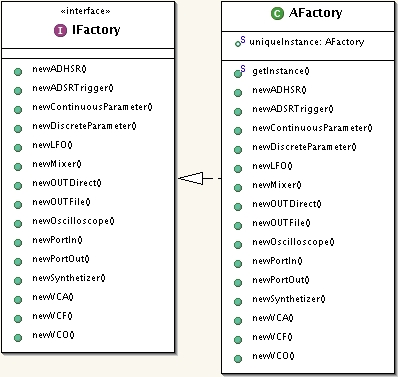
\includegraphics[scale=0.5]{img/moteur/Afactory.jpg}
		\caption{Diagramme de la fabrique de composants applicatifs du package \code{core}}
		\label{actionButton-ai}
	\end{center}
\end{figure}

La plupart des �l�ments du c\oe ur sont dans le paquetage \emph{core}.

\begin{figure}[!h]
	\begin{center} 
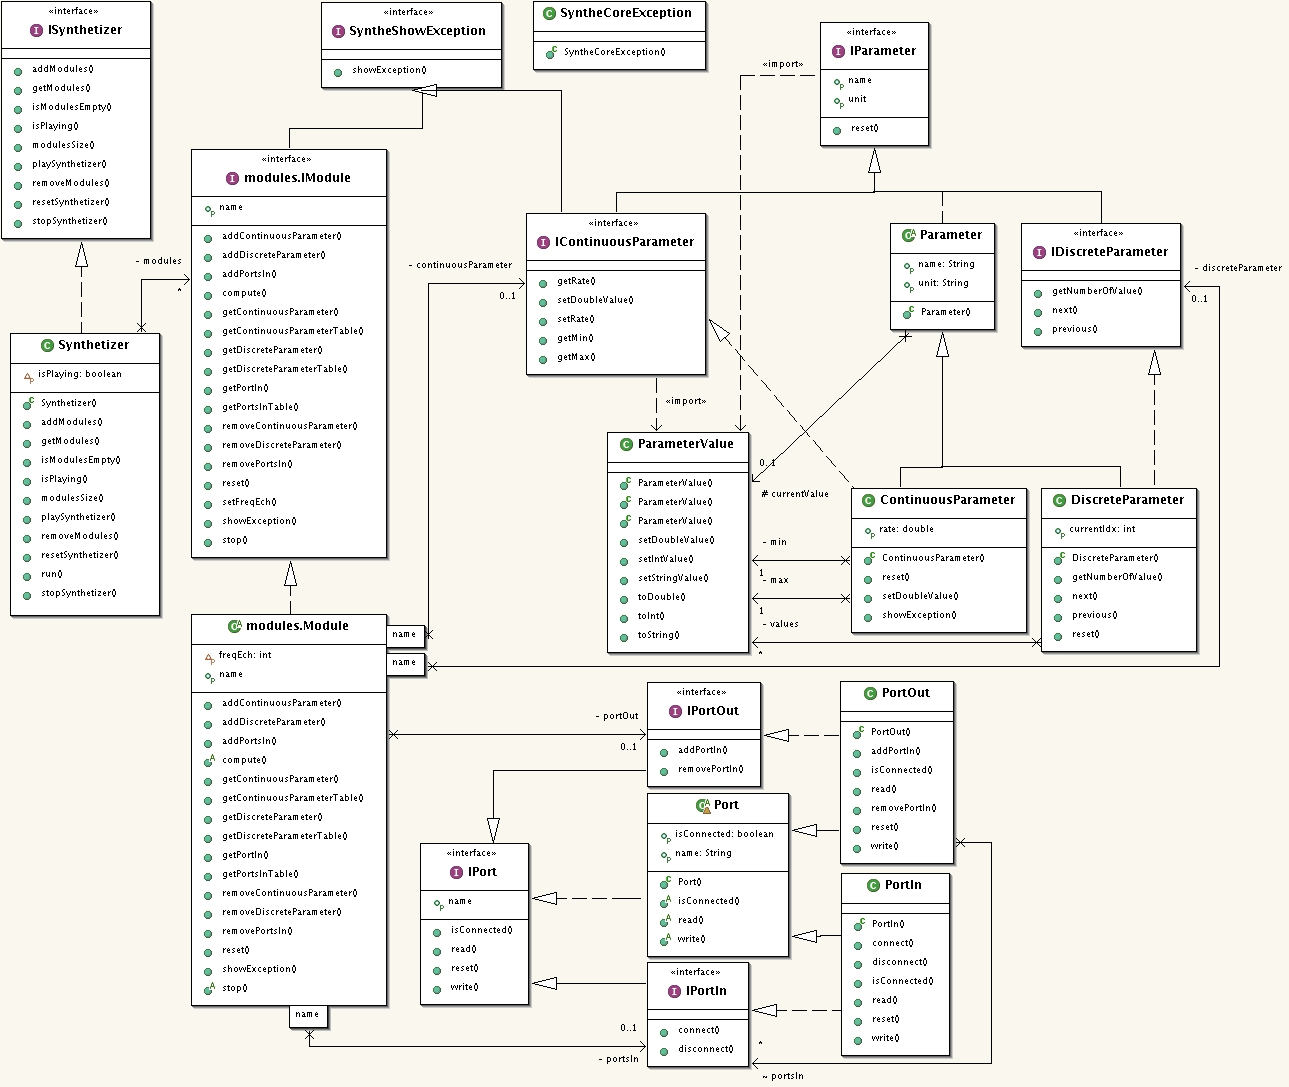
\includegraphics[scale=0.3]{img/moteur/core-ai.jpg}
		\caption{Diagramme des �l�ments du coeur : \code{core}}
		\label{core-ai}
	\end{center}
\end{figure}

\newpage

\subsubsubsection{Package core.modules}

Les modules sont la partie du logiciel qui contiennent les algorithmes g�n�rant 
et traitant le signal sonore.

\begin{figure}[!h]
	\begin{center} 
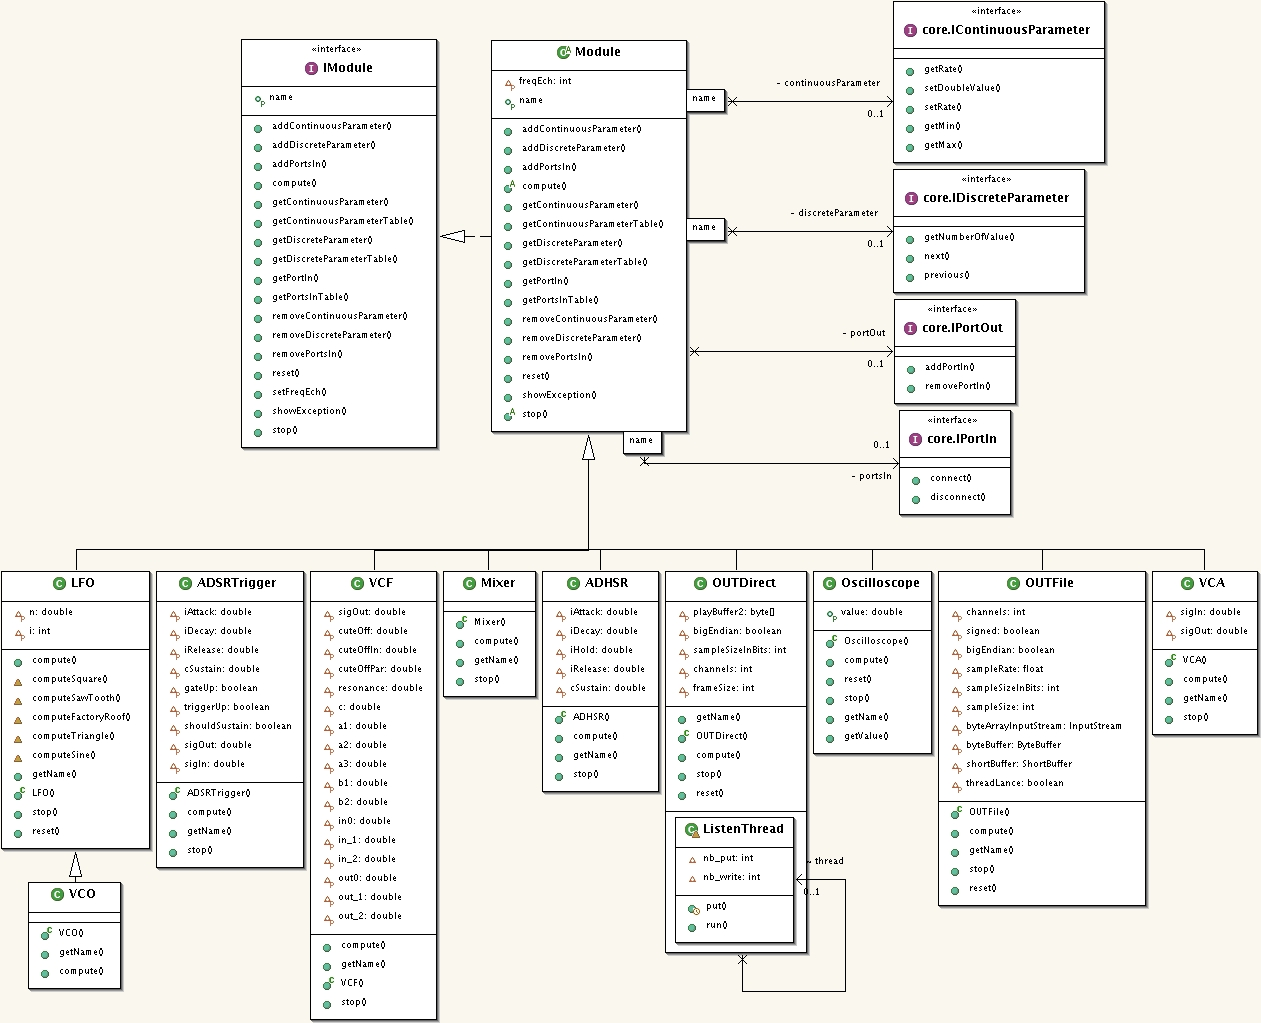
\includegraphics[scale=0.3]{img/moteur/modules-ai.jpg}
		\caption{Diagramme des modules : \code{core.modules}}
		\label{modules-ai}
	\end{center}
\end{figure}

\subsubsection{Diagrammes de s�quence}

\begin{figure}[!h]
	\begin{center} 
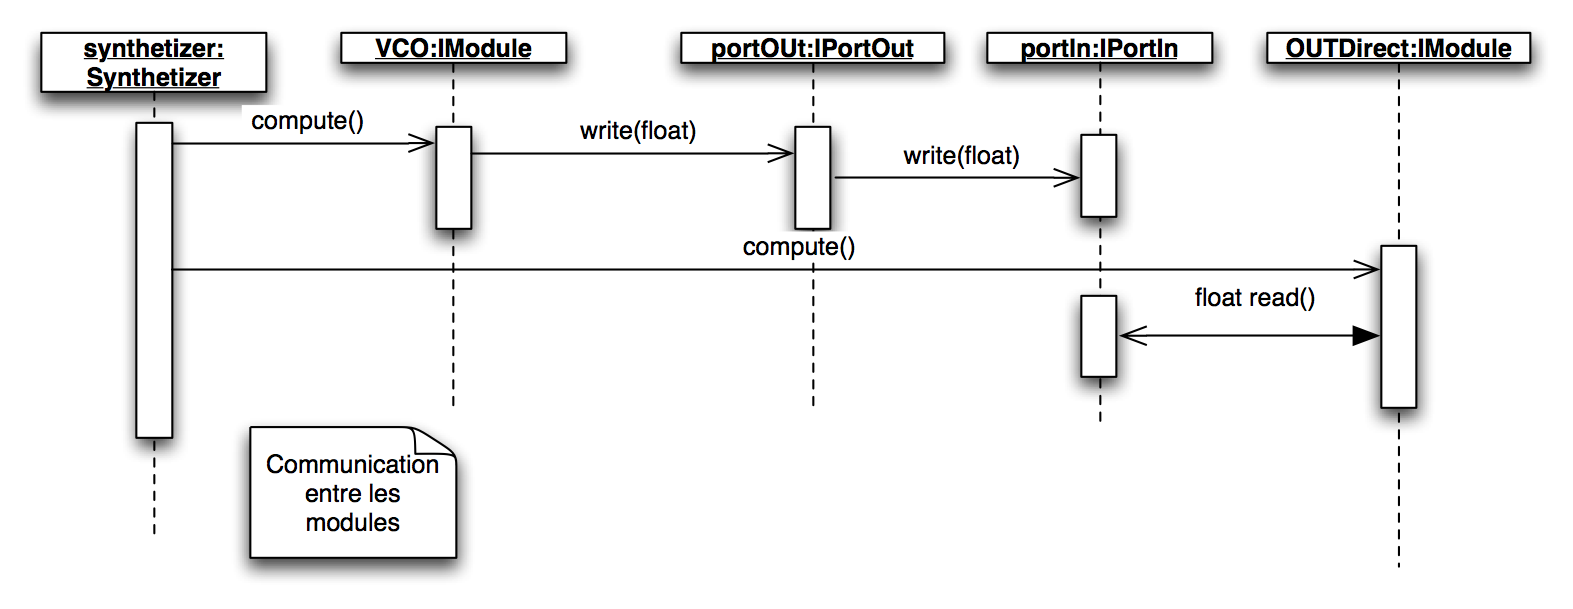
\includegraphics[scale=0.25]{img/moteur/communication_modules.png}
		\caption{Diagramme de s�quence : \code{core.modules}}
		\label{communication-modules}
	\end{center}
\end{figure}



\newpage
\section{Mod\`ele d'architecture PAC} \label{pac}

Un des objectifs du projet est de rendre interactif chaque composant applicatif 
du mod\`ele m\'etier d\'evelopp\'e tout en  veillant  \`a ce que les parties 
``Synth\`ese audio'' et ``Interface graphique'' soient bien s\'epar\'ees.

Afin de respecter � cette contrainte, il n\'ecessaire de mettre en place un 
proxy qui va \^etre un composant dont le r\^ole sera premi\`erement d'assurer 
l'acc\`es au composant applicatif et deuxi\`ement, de r\'epercuter les 
modifications du composant applicatif via un composant de pr\'esentation. 
\bigskip

Le choix du mod\`ele d'architecture \index{PAC} PAC  \cite{duval} se r\'ev\`ele donc 
judicieux. En le respectant au maximum, la s\'eparation entre le mod\`ele 
m\'etier et l'interface graphique est facilit�e.

Le mod\`ele PAC s'articule autour d'une entit\'e de base nomm\'ee agent PAC. 
Chaque agent se d\'ecoupe en trois facettes :
\begin{itemize}
\item Pr\'esentation. \index{PAC!presentation@Pr�sentation}
\item Abstraction. \index{PAC!abstraction@Abstraction}
\item Contr�le. \index{PAC!controle@Contr�le}
\end{itemize}

Le composant servant de proxy se substitue \`a la facette Contr\^ole, le 
composant applicatif \`a la facette Abstraction, et le composant de 
pr\'esentation \`a la facette Pr\'esentation. \bigskip

%*****************************************

\subsection{Mise en oeuvre du mod\`ele PAC}
Les composants de contr�le de l'application sont construits � partir du patron 
\code{Proxy} \index{Design Pattern!Proxy}.

\begin{figure}[h!] \centering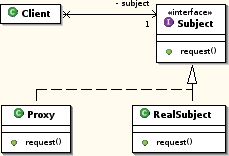
\includegraphics[scale=1.0]{img/pac/proxy.png}
\caption{Patron de conception \code{Proxy}}
\end{figure}

Le composant de contr\^ole remplace le composant applicatif aux vues des autres 
composants. Il assure la coh\'erence entre son composant applicatif et son 
composant de pr\'esentation.

\newpage

 Les services propos\'es par les composants applicatifs du mod\`ele m\'etier 
 sont d\'efinis par l'interm\'ediaire d'interfaces impl\'ement\'ees par chacun 
 d'entre eux. On s'inspire alors du design pattern \code{Template Method} 
 \index{Design Pattern!Template Method}.

\begin{figure}[h!] 
\centering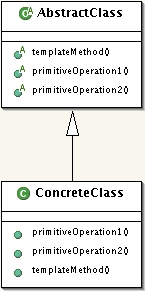
\includegraphics[scale=0.55]{img/pac/template_method.jpg}
\caption{Patron de conception \code{Template Method}}
\end{figure}

Ce patron force la d�finition de l'interface d'acc\`es de chaque composant. Il 
permet aussi de d\'ecoupler  le composant de contr�le de son composant 
applicatif et de son composant de pr�sentation.  \bigskip
 
En appliquant au mod\`ele PAC les deux patrons d\'ecrits pr\'ec\'edemment on 
obtient les composants PAC suivants :

\begin{figure}[h!] 
\begin{center}
	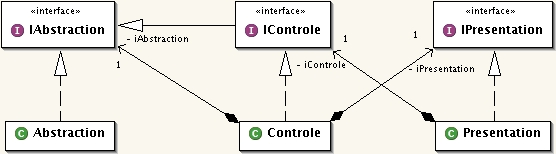
\includegraphics[scale=0.6]{img/pac/pac.jpg}
	\caption{mod\`ele PAC et proxy contr�le par d\'el\'egation}
\end{center}
\end{figure}

\begin{description}
\item [Remarque ]:\\  Conform�ment au patron \code{Proxy}, chaque composant de 
contr�le doit impl�menter l'interface du composant applicatif auquel il est 
rattach�. L'interface du composant de contr�le h�rite donc de l'interface du 
composant applicatif.
\item[Notations ]:\\ Le nom de l'interface d�finissant les services rendus par 
un composant donn� est pr�fix� par la lettre \verb+I+ suivie du nom du 
composant applicatif.

Le nom de la classe impl�mentant le contr�le d'un composant applicatif est 
pr�fix� par la lettre \verb+C+ suivie du nom du 
composant applicatif.

Enfin, le nom de la classe impl�mentant la pr�sentation d'un composant 
applicatif est pr�fix� par la lettre \verb+P+ suivie du nom du composant applicatif.
\end{description}
\bigskip

Le mod�le d'architecture retenu facilite l'utilisation de fabriques de 
composants. Les fabriques ont pour avantage de rendre les composants 
interactifs les plus ind\'ependants possibles des composants applicatifs. Elles 
sont impl\'ement\'ees sur la base du patron \code{Abstract Factory} 
\index{Design Pattern!Abstract Factory}.

\begin{figure}[h!] 
	\begin{center}
		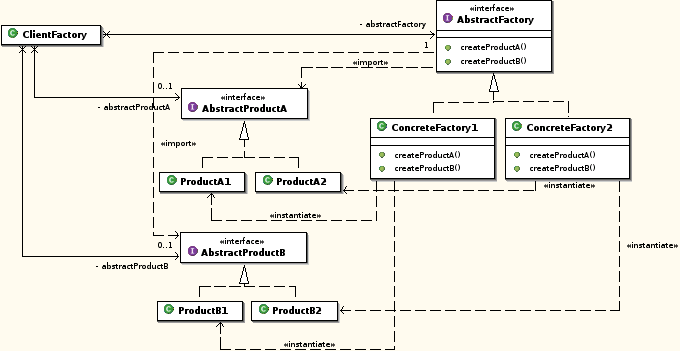
\includegraphics[scale=1.0]{img/pac/abstract_factory.png}
		\caption{Patron de conception \code{Abstract Factory}}
	\end{center}
\end{figure}

Une premi�re fabrique (\code{core.AFactory}) est consacr�e � la cr�ation des 
composants applicatifs et est utilis�e dans les composants de contr�le 
associ�s. Une seconde fabrique (\code{gui.controle.CFactory}) est consacr�e � 
la cr�ation des composants de contr�le. Ces deux fabriques impl�mentent lae m�me 
interface (\code{IPFactory}). La seconde fabrique permet alors de substituer � 
chaque composant applicatif son composant proxy associ�.

Enfin une troisi�me fabrique (\code {gui.presentation.PFactory}) permet de 
cr�er les composants de pr�sentation et est utilis�e dans les composants de 
contr�le afin d'associer une abstraction � la pr�sentation correspondante.

\newpage Chaque fabrique de composants impl\'emente en plus le patron 
\code{Singleton} \index{Design Pattern!Singleton}.

\begin{figure}[h!] \centering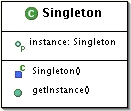
\includegraphics[scale=0.7]{img/pac/singleton.jpg}
\caption{Patron de conception \code{Singleton}}
\end{figure}

Ce patron va permettre d'assurer qu'une seule instance de chacune des fabriques 
est instanci\'ee pendant toute la dur\'ee de l'application.

%*****************************************

\subsection{Composants applicatifs}\index{Composants applicatifs}
Les composants applicatifs sont pr�sent�s dans la section \ref{moteur audio} 
page \pageref{moteur audio}.

\subsection{Composants de pr�sentation}\index{composants de presentation@Composants de pr�sentation}
Les classes impl�mentant les pr�sentations des composants applicatifs sont 
regroup�s dans le package \code{gui.presentation}.

Ce package regroupe � la fois les interfaces des pr�sentations et les classes 
impl�mentant ces interfaces. Il poss�de dix interfaces :
\begin{description}
    \item [IPFactory] : D�crit les m�thodes permettant de cr�er les 
    pr�sentations des composants applicatifs.
    \item [IPPort] :  D�crit les pr�sentations des classes h�ritant de
    \code{core.Port}
    \item [IPPortIn] : H�rite de \code{IPPort} et d�crit la pr�sentation 
    de \code{core.PortIn}.
    \item [IPPortOut] : H�rite de \code{IPPort} et d�crit la pr�sentation 
    de \code{core.PortOut}.
    \item [IPParameter] : D�crit les pr�sentations des classes h�ritant de 
    \code{core.Parameter}.
    \item [IPDiscreteParameter] : H�rite de \code{IPParameter} et d�crit 
    la pr�sentation de \\
\code{core.DiscreteParameter}.
      \item [IPContinuousParameter] : H�rite de \code{IPParameter} et 
      d�crit la pr�sentation de \\
\code{core.ContinuousParameter}.
    \item [IPModule] : D�crit la pr�sentation des classes h�ritant de 
      \code{core.modules.Module}.
    \item [IPOscilloscope] : H�rite de \code{IPModule} et d�crit la 
      pr�sentation de \\
\code{core.modules.Oscilloscope}.
    \item [IPSynthetizer] : D�crit la pr�sentation de 
      \code{core.Synthetizer}.
\end{description}

\newpage Le diagramme ci-dessous pr�sente les interfaces ainsi que les liens 
entre les diff�rentes classes du package.

\begin{figure}[h!] 
\begin{center} 
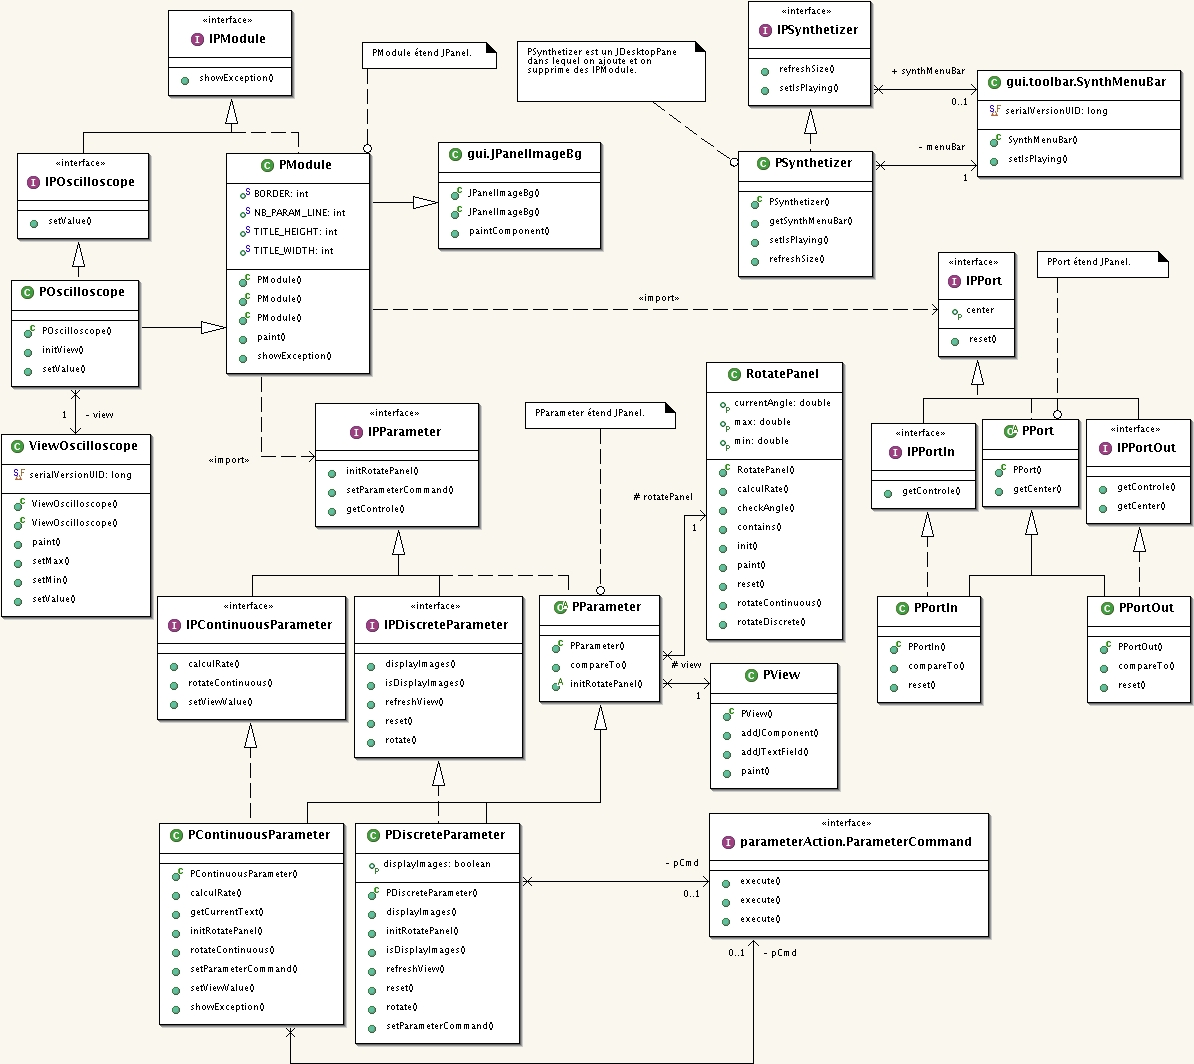
\includegraphics[scale=0.4]{img/pac/presentation-ai.jpg}
\caption{Composants de pr�sentation}
\end{center}
\end{figure}
\newpage

\subsubsection{PFactory}
\code{PFactory} impl�mente \code{IPFactory}, c'est la fabrique de composants de 
pr�sentation du package \code{gui.presentation}. Elle est utilis�e pour 
d�coupler le contr�le de la pr�sentation.

\subsubsection{PPortIn et PPortOut}
\code{PPortIn} et \code{PPortOut} h�ritent de
\code{PPort} et impl�mentent respectivement \code{IPPortIn} 
et \code{IPPortOut}. \code{PPort} impl�mente \code{IPPort} et �tend 
\code{JPanel}. Elle d�finit l'aspect graphique d'un port d'entr�e ou de sortie.

\code{PPortIn} est une zone sur laquelle on peut effectuer un drop. Le drop est 
activ� dans le constructeur de la mani�re suivante :
\begin{verbatim}
dropper = new ConnectorDropper(this); 
dropper.activerDropListener();
\end{verbatim}

\code{PPortOut} est une zone sur laquelle on peut effectuer un drag. Le drag 
est activ� dans le constructeur de la mani�re suivante :
\begin{verbatim}
dragger = new ConnectorDragger(this); 
dragger.activerDragListener();
\end{verbatim}

Le drag'n drop est ici utilis� pour connecter un port de sortie � un port 
d'entr�e (plus de d�tails dans la section \ref{interface} page 
\pageref{interface}).

\subsubsection{PDiscreteParameter et PContinuousParameter}
\code{PDiscreteParameter} et \code{PContinuousParameter} h�ritent de 
\code{PParameter}, et impl�mentent respectivement \code{IPDiscreteParameter} et 
\code{IPContinuousParameter}. Leur aspect graphique est identique : il s'agit 
d'un bouton que l'on peut tourner dans les deux sens.

La classe \code{PParameter} impl�mente \code{IPParameter} et 
�tend \code{JPanel}. Elle d�finit les m�thodes communes aux deux classes et 
place les diff�rents objets graphiques qui les composent.

Le comportement du bouton est diff�rent dans les deux classes : il tourne cran par 
cran pour \code{PDiscreteParameter} et tourne d'un minimum vers un maximum pour 
\code{PContinuousParameter}. \bigskip

\code{PParameter} poss�de  une variable d'instance de  type 
\code{RotatePanel}. \code{RotatePanel} permet d'effectuer une rotation sur une image. 
La rotation est d�finie suivant trois angles : un minimum, un maximum et un 
angle courant. Les classes \code{PDiscreteParameter} et \code{PContinuousParameter} 
agissent sur la rotation de l'image via les m�thodes respectives 
\code{rotateDiscrete(boolean sens)} et \code{rotateContinuous(double f)} o� 
\code{f} repr�sente un pourcentage.

Une variable d'instance de type \code{PView} affiche de mani�re format�e des 
informations sous forme de \code{JTextComponent}. \code{PDiscreteParameter} 
affiche soit des chaines de caract�res, soit des images, via des \code{JLabel}. 
\code{PContinuousParameter} affiche des cha�nes de caract�res (valeur et unit� 
de mesure) et autorise une saisie, via un \code{JTextField}.

Enfin, une variable d'instance de type
\code{gui.}\code{presentation.}\\\code{parameterAction.}\code{ParameterCommand} 
d�finit le code � ex�cuter lors d'une action de l'utilisateur sur cette 
pr�sentation.

\subsubsection{PModule}
\code{PModule} impl�mente \code{IPModule} et �tend \code{JPanel}. Un des 
objectifs fix�s en d�but de projet est de ne pas cr�er de pr�sentation 
sp�cifique pour chaque type de module impl�ment� dans le package 
\code{core.modules}.

\code{PModule} est donc une pr�sentation param�trable respectant cette 
contrainte.

Les trois contructeurs de la classe sont les suivants :
\begin{tabbing} 
\hspace{0.7cm} \=  \\
\code{public PModule(ICModule controle)} \\
\> Constructeur principal. \\
\code{public PModule(Collection<IPParameter> params, Collection<IPPort> pIn,}\\
\> \code{ICModule controle)} \\
\> Constructeur pour les modules sans port de sortie -- utilise le constructeur \\
\> pr�c�dent. \\
\code{public PModule(Collection<IPParameter> params, Collection<IPPort> pIn,} \\
\> \code{IPPort pOut, ICModule controle)}\\
\> Constructeur pour les modules avec un port de sortie -- utilise le constructeur\\
\> pr�c�dent.
\end{tabbing}


Les param�tres d'entr�e des constructeurs sont pr�cis�s ci-dessous :

\begin{itemize}
  \item \code{params} : les pr�sentations des param�tres discrets et continus 
  d'un module.
  \item \code{pIn} : les pr�sentations des ports d'entr�e d'un module.
  \item \code{pOut} : la pr�sentation du port de sortie d'un module.
  \item  \code{controle} : le contr�le du module.\bigskip
\end{itemize}

Tous les objets graphiques composant la pr�sentation des modules sont 
positionn�s dynamiquement et en fonction de leur taille.\bigskip

Les avantages procur�s par cette pr�sentation g�n�rique sont les suivants :
\begin{enumerate}
  \item Pas de couplages avec la pr�sentation des ports et des param�tres des 
  modules.
  \item Si on ajoute un nouveau module conforme � \code{core.IModule}, il n'y a 
  pas besoin de lui d�finir une pr�sentation sp�cifique.
  \item On peut �tendre la classe si on veut ajouter une pr�sentation 
  particuli�re.
  \item Gain de temps.\medskip
\end{enumerate}

Les inconv�nients de cette pr�sentation :
\begin{enumerate}
  \item Couplage fort avec l'API javax.Swing.
\end{enumerate}

\subsubsection{PSynthetizer}
Cette classe impl�mente \code{IPSynthetizer} et �tend \code{JDesktopPane}.

Elle constitue le plan de travail dans lequel les diff�rentes pr�sentations de 
modules vont �tre ajout�es, supprim�es.

C'est via cette pr�sentation que l'utilisateur peut lancer la simulation en 
temps r�el et interagir avec le mod�le m�tier.

\subsection{Composants de contr\^ole}\index{composants de controle@Composants de contr�le}
Les classes impl�mentant les contr�les des composants applicatifs sont 
regroup�s dans le package \code{gui.controle}.

Ce package est ind�pendant de l'impl�mentation choisie pour les composants 
applicatifs et de pr�sentation. Il les conna�t uniquement via leurs interfaces. 
Il contient donc la liste des interfaces des composants de contr�le ainsi que 
les classes qui les impl�mentent.

L'interface d'un composant de contr�le h�rite de l'interface du composant 
applicatif correspondant. On y ajoute cependant la d�claration d'une m�thode 
suppl�mentaire permettant de r�cup�rer le composant de pr�sentation auquel il 
est associ�.

Les interfaces contenues dans ce package sont les suivants :
\begin{itemize}
    \item \code{ICPortIn} : H�rite de \code{IPortIn} et d�crit le contr�le  de \code{core.PortIn}.
    \item \code{ICPortOut} : H�rite de \code{IPortOut} et d�crit le contr�le  de \code{core.PortOut}.
    \item \code{ICParameter} : H�rite de \code{IParameter} et d�crit les contr�les des classes h�ritant de 
    \code{core.Parameter}.
    \item \code{ICDiscreteParameter} : H�rite de \code{ICParameter} et d�crit 
    le contr�le  de 
    
      \code{core.DiscreteParameter}.
      \item \code{ICContinuousParameter} : H�rite de \code{ICParameter} et 
      d�crit le contr�le  de 
      
        \code{core.ContinuousParameter}.
      \item \code{ICModule} : H�rite de \code{IModule} et d�crit les contr�les  des classes h�ritant de 
      \code{core.modules.Module}.
      \item \code{ICSynthetizer} : H�rite de \code{ISynthetizer} et d�crit le contr�le  de 
      
      \code{core.Synthetizer}.
\end{itemize}

\begin{description}
\item[Remarque] : Il n'est pas n�cessaire de d�finir une interface pour une nouvelle fabrique de composants de contr�le.
L'interface utilis�e est \code{core.IFactory}.
\end{description}

\subsubsection{CFactory}
\code{CFactory} impl�mente \code{IFactory}, c'est la fabrique de composant de 
contr�le. Cette fabrique impl�mente le m�me interface que la fabrique de 
composants applicatifs \\ \code{core.AFactory}. Ceci nous permet de substituer 
les composants de contr�le aux composants applicatifs.

\newpage
\subsubsection{CPortIn et CPortOut}
\code{CPortIn} et \code{CPortOut} impl�mentent respectivement les interfaces 
\code{ICPortIn} et \code{ICPortOut} comme on peut le voir sur les diagrammes ci-dessous.

\begin{figure}[h!] 
\centering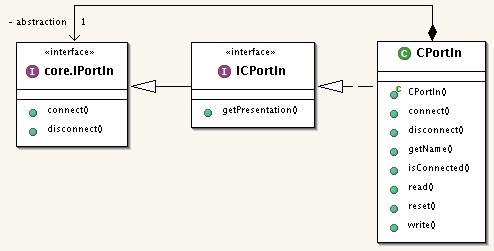
\includegraphics[scale=0.6]{img/pac/controle_port_in.png}
\center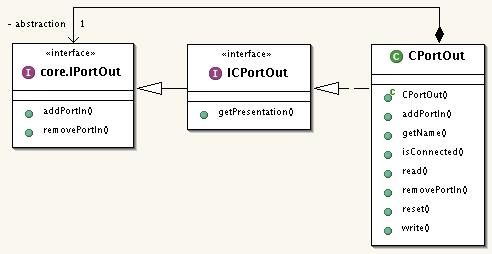
\includegraphics[scale=0.6]{img/pac/controle_port_out.png}
\caption{Diagramme de classe contr�le des PortIn et PortOut}
\end{figure}

Ces deux classes ne servent que de relais, il n'y a pas de traitement particulier � 
r�aliser lors d'une modification de l'abstraction.

Le constructeur de \code{CPortIn} illustre bien la mani�re dont les composants de contr�le du package cr�ent leur abstraction et leur pr�sentation.
{\small
\begin{verbatim}
public CPortIn(String name) {
    abstraction = ConcreteFactory.getAFactory().newPortIn(name);
    presentation = ConcreteFactory.getPFactory().newPPortIn(name, this);
}
\end{verbatim}
}

\newpage
\subsubsection{CContinuousParameter et CDiscreteParameter}
\code{CContinuousParameter} et \code{CDiscreteParameter} impl�mentent respectivement les interfaces 
\code{IContinuousParameter} et \code{ICDiscreteParameter}.

\begin{figure}[h!] \centering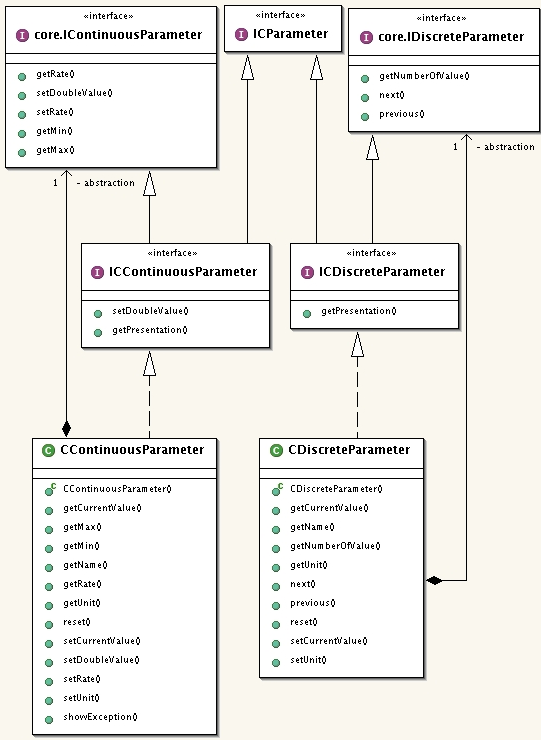
\includegraphics[scale=0.6]{img/pac/controle_parameter.png}
\caption{Diagramme de classe contr�le des ContinuousParameter et DiscreteParameter}
\end{figure}
\newpage

L'utilisateur peut interagir avec les pr�sentations de ces deux contr�les. Ces derniers 
doivent donc maintenir la coh�rence entre l'abstraction et la pr�sentation.

Les exemples suivants pr�sentent le m�canisme 
mis en \oe uvre dans les contr�les afin d'assurer cette coh�rence.
\bigskip

{\bf Exemple -- classe \code{CDiscreteParameter}} : 
{\small
\begin{verbatim}
public ParameterValue previous() {
    ParameterValue tmp = abstraction.previous();
    presentation.refreshView(tmp.toString());
    presentation.rotate(false);
    return tmp;
}
\end{verbatim}
}

{\bf Exemple -- classe \code{CContinuousParameter}} : 
{\small
\begin{verbatim}
public void setDoubleValue(double value) {
    abstraction.setDoubleValue(value);
    presentation.rotateContinuous(abstraction.getRate());
    presentation.setViewValue(abstraction.getCurrentValue().toString());
}
\end{verbatim}
}

\subsubsection{CModule}
\code{CModule} est une classe abstraite impl�mentant \code{ICModule}. Toutes les 
m�thodes d�clar�es dans \code{IModule} et dans \code{ICModule} sont r�ellement 
impl�ment�es dans \code{CModule} et pas seulement d�clar�es.

La pr�sentation des modules n'interagit pas avec le mod�le m�tier, les 
contr�les des modules d�l�gant les traitements � leur abstraction.

Les sous-classes de \code{CModule} (CVCA, CVCO, CLFO, etc$\ldots$) sont 
utilis�es uniquement pour impl�menter des traitements sp�cifiques pour chacun 
des modules du package \code{core}, si besoin est. Il suffit alors de 
surcharger une des m�thodes h�rit�es de \code{CModule}.

\newpage

Des traitements communs � tous les contr�les de module sont r�alis�s lors de 
leur cr�ation. Afin de factoriser au mieux le code, \code{CModule} impl�mente 
un constructeur g�n�rique  : {\small \code{public CModule(IModule abstraction)}}.
Ce constructeur accepte en param�tre l'abstraction d'un contr�le de type \code{IModule}.

Les sous-classes appels ensuite le constructeur de \code{CModule} comme dans 
l'exemple suivant : 
{\small
\begin{verbatim}
public class CLFO {
    public CLFO() { 
        super(ConcreteFactory.getAFactory().newLFO()); 
    }
    ...
}
\end{verbatim}

Certains contr�les doivent pouvoir param�trer les pr�sentations de leurs 
param�tres discrets. La m�thode abstraite 
\code{addPDiscreteParameters(Hashtable<String, DiscreteParameter> 
discreteParameters)} d�finie dans \code{CModule} doit �tre impl�ment�e dans 
chaque sous-classe. Soit cette m�thode ne fait rien soit elle r�alise un 
traitement sur les param�tres discrets comme dans l'exemple suivant :

{\footnotesize
\begin{verbatim}
public class CLFO {
    ...
    public void addPDiscreteParameters(
    		Hashtable<String, IDiscreteParameter>discreteParameters) {
        ICDiscreteParameter shape = 
        	(ICDiscreteParameter)discreteParameters.get(LFO.PARAM_SHAPE); 
        shape.getPresentation().displayImages(); 
    }
    ...
 }
\end{verbatim}
}

La m�thode \code{createPresentation(ArrayList<IPParameter> pParams, ArrayList<IPPort> pports, IPortOut po, CModule module)} permet de 
red�finir la pr�sentation par d�faut d'un module. 
Cette pr�sentation doit cependant �tre de type \code{IPModule}.

L'exemple suivant pr�sente l'utilisation de cette m�thode pour le contr�le \code{COscilloscope} pour lequel une pr�sentation diff�rente � �t� cr��e :
{\footnotesize
\begin{verbatim}
public class {
    ...
    protected void createPresentation(ArrayList<IPParameter> pParams, 
                               ArrayList<IPPort> pports, IPortOut po, CModule module) { 
        presentation = ConcreteFactory.getPFactory().newPOscilloscope(pports.get(0),this); 
    }
}
\end{verbatim}
}

\newpage

\begin{figure}[h!] \centering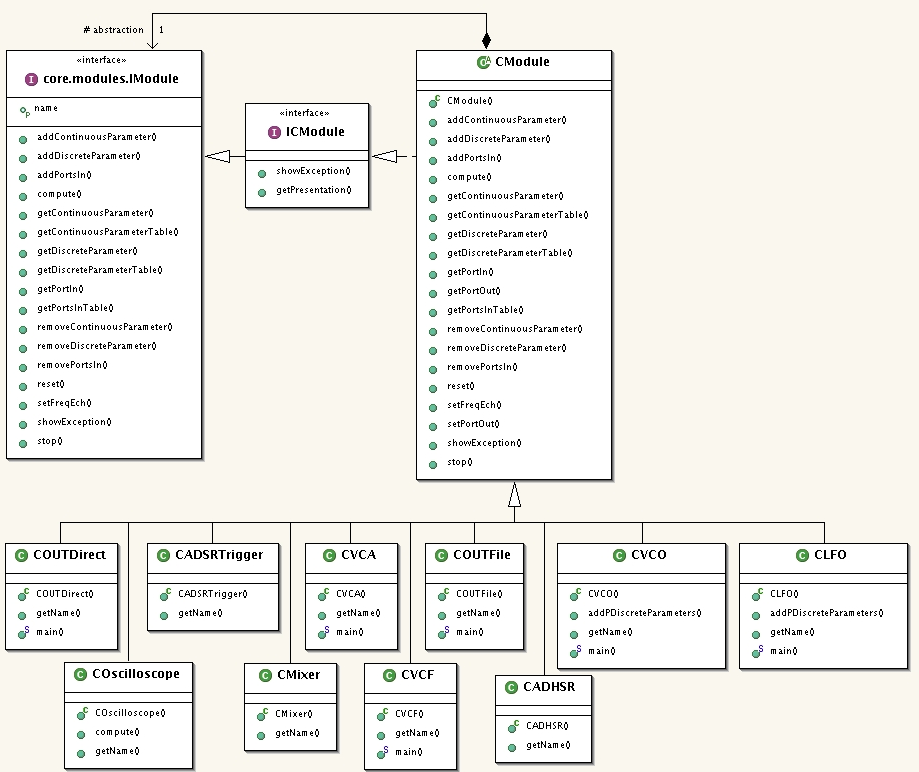
\includegraphics[scale=0.5]{img/pac/controle_module.png}
\caption{Diagramme de classe contr�le CModule}
\end{figure}
\newpage

\subsubsection{CSynthetizer}
\code{CSynthetizer} impl�mente \code{ICSynthetizer}.

 \begin{figure}[h!] \centering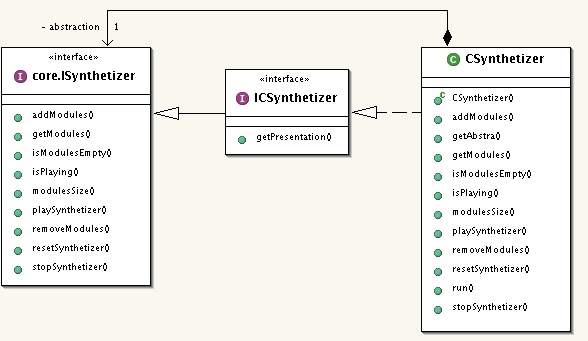
\includegraphics[scale=0.6]{img/pac/controle_synthe.png}
\caption{Diagramme de classe contr�le Synthetizer}
\end{figure}

\code{CSynthetizer} ne fait principalement que d�l�guer les traitements � son 
abstraction, � l'exception des deux traitements ci-dessous :
\begin{verbatim}
public void playSynthetizer() {
   abstraction.playSynthetizer(); 
   presentation.setIsPlaying(abstraction.isPlaying());
}
public void stopSynthetizer() {
   abstraction.stopSynthetizer(); 
   presentation.setIsPlaying(abstraction.isPlaying());
}
\end{verbatim}





%*****************************************

\subsection{Fabriques de composants}


\code{ConcreteFactory} est la classe permettant d'acc�der aux diff�rentes fabriques de composants.
Cette classe propose quatre m�thodes pour obtenir les diff�rentes fabriques : 
\begin{description}
  \item [\code{getAFactory}] :
  
Elle permet � un contr�le d'obtenir la fabrique des composants applicatifs.
  \item [\code{getCFactory}] : 
  
Elle permet � un contr�le d'obtenir la fabrique des composants de contr�le.  
  \item [\code{getPFactory}] : 
  
Elle permet � un contr�le d'obtenir la fabrique des composants de pr�sentation.
  \item [\code{getFactory}] : 
  
Elle est utilis� par une abstraction et retourne une \code{CFactory} si une 
\code{CFactory} a �t� instanci�e, ou une \code{AFactory} par d�faut.
\end{description}

\newpage

\begin{figure}[h!] \centering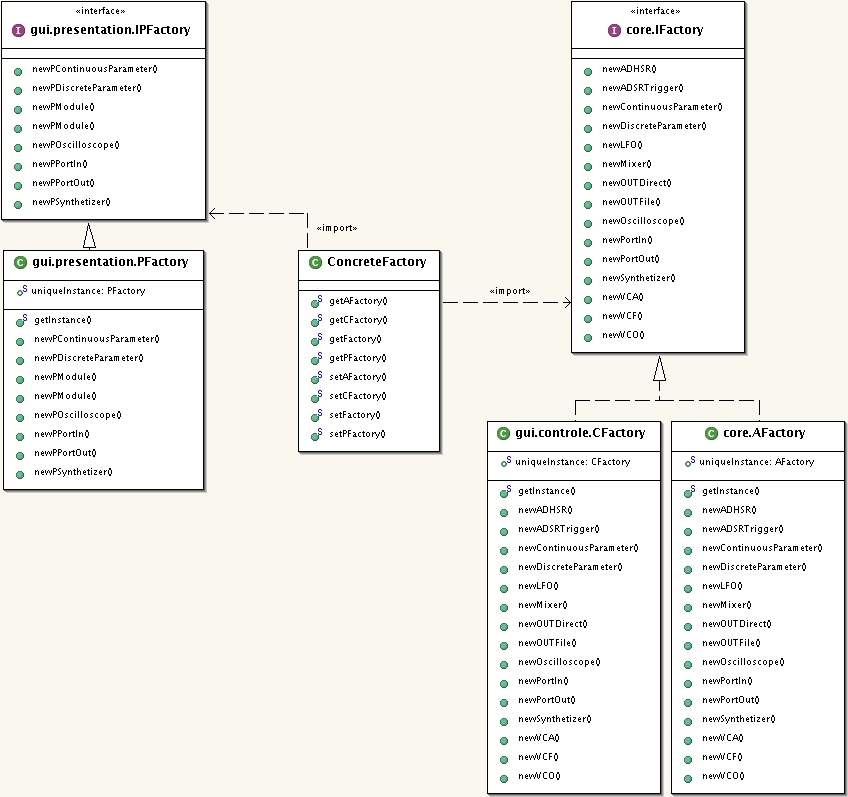
\includegraphics[width=\textwidth]{img/pac/concreteFactory-aid.jpg}
\caption{Fabriques de composants}
\end{figure}

\newpage

%*****************************************

\subsection{Diagrammes UML des composants PAC d\'evelopp\'es.}

\subsubsection{Composant PAC Synthetizer}
\begin{figure}[h!] \centering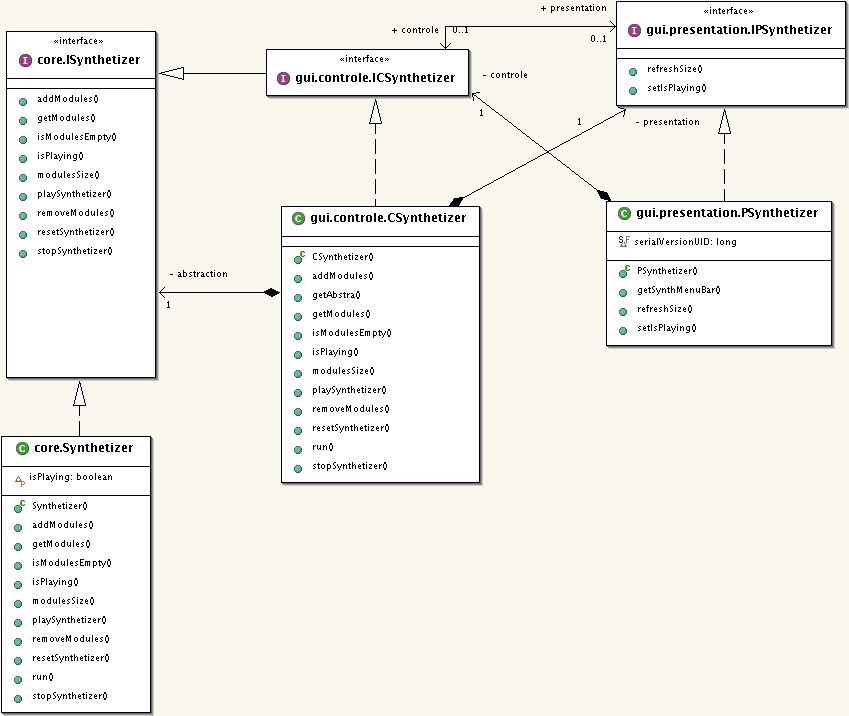
\includegraphics[width=\textwidth]{img/pac/pac_synthe.jpg}
\caption{Composant PAC Synthetizer}
\end{figure}
\newpage

\subsubsection{Composant PAC Module}
\begin{figure}[h!] \centering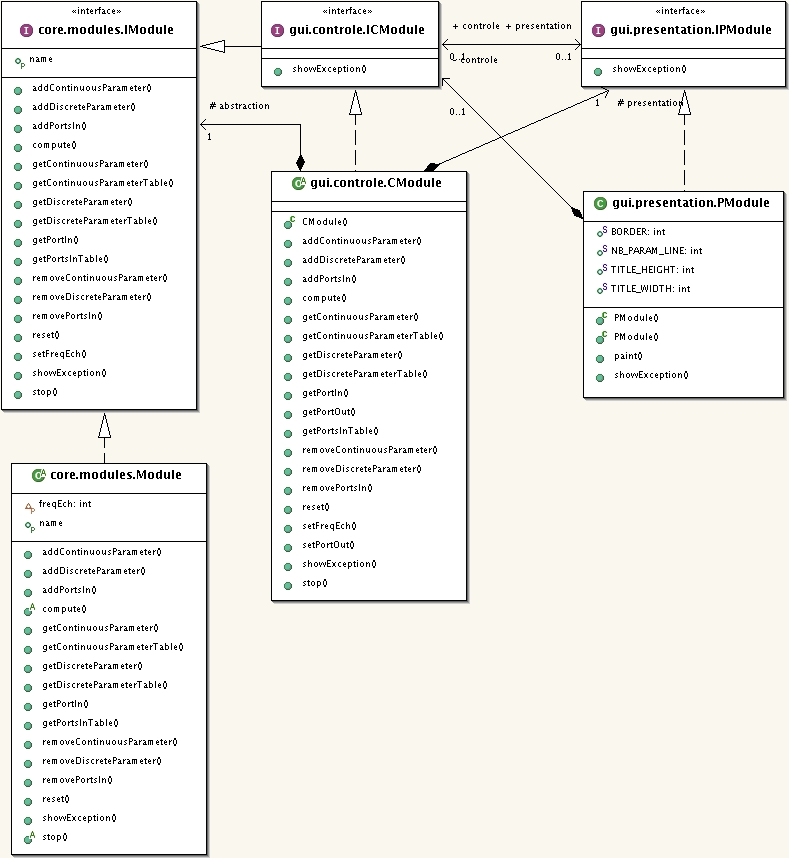
\includegraphics[width=\textwidth]{img/pac/pac_module.jpg}
\caption{Composant PAC Module}
\end{figure}
\newpage

\subsubsection{Composant PAC Oscilloscope}
\begin{figure}[h!] 
\centering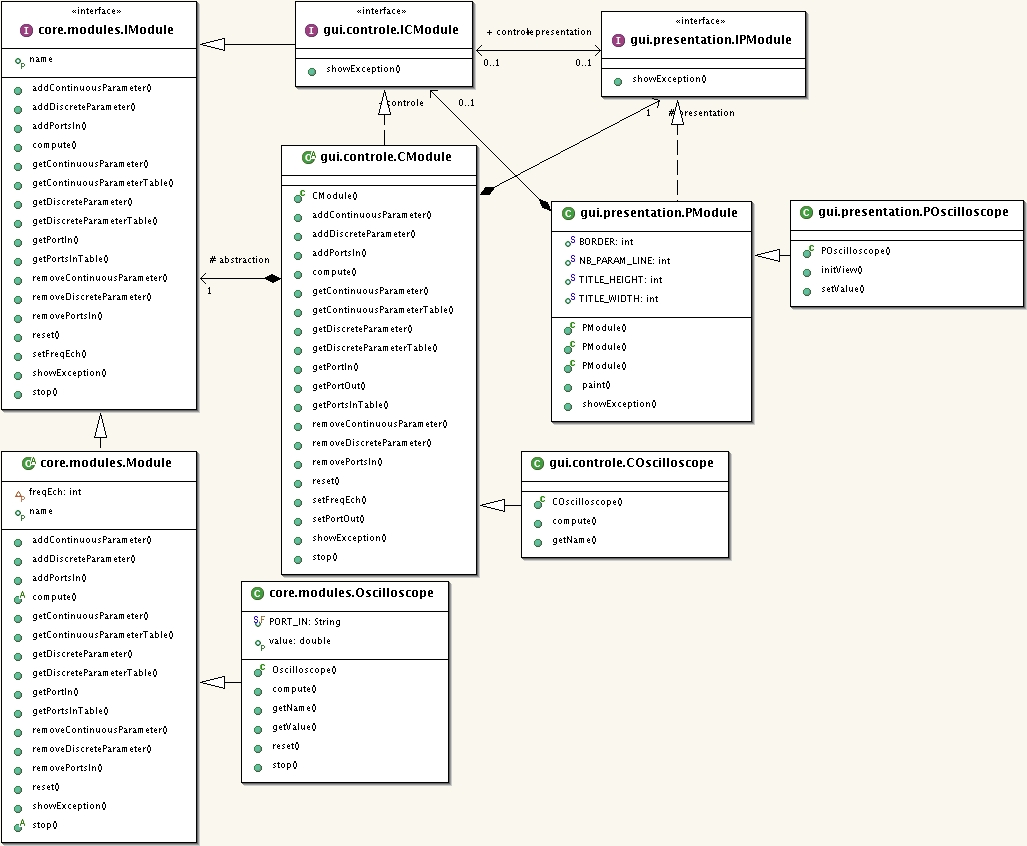
\includegraphics[width=\textwidth]{img/pac/pac_oscilloscope.jpg}
\caption{Composant PAC Oscilloscope}
\end{figure}
\newpage

\subsubsection{Composant PAC DiscreteParameter}
\begin{figure}[h!] 
\centering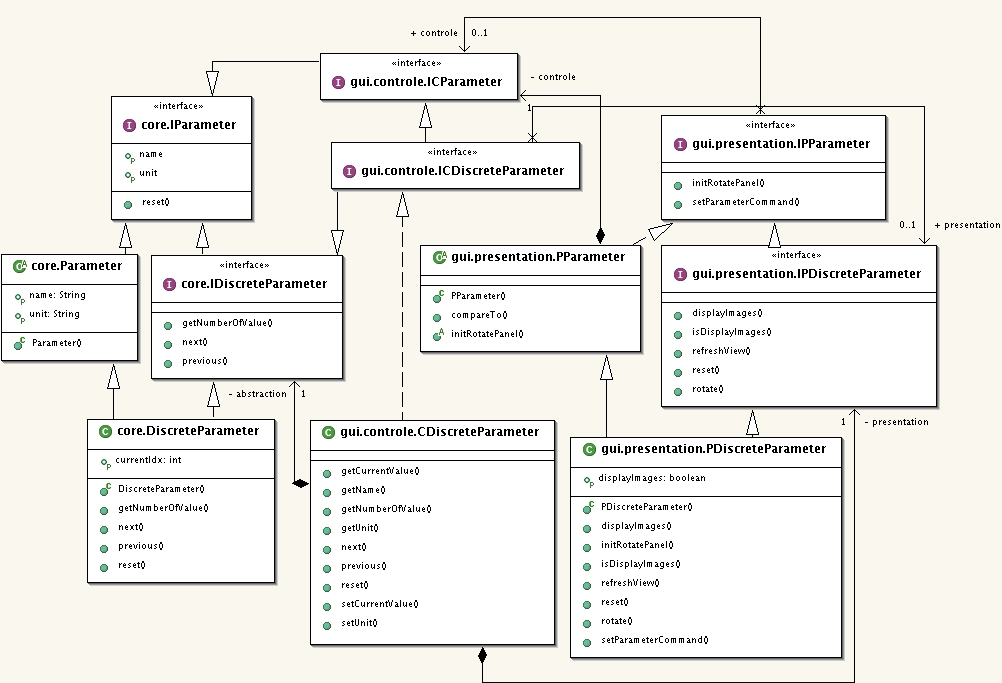
\includegraphics[width=\textwidth]{img/pac/pac_discreteParameter.jpg}
\caption{Composant PAC DiscreteParameter}
\end{figure}
\newpage

\subsubsection{Composant PAC ContinuousParameter}
\begin{figure}[h!] 
\centering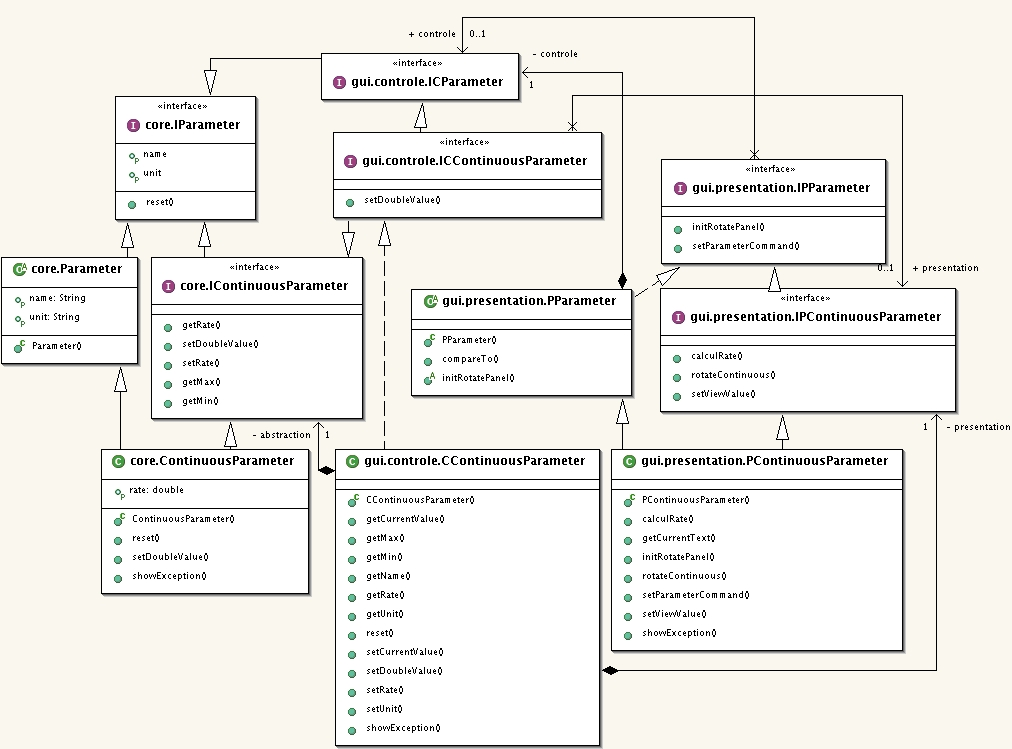
\includegraphics[width=\textwidth]{img/pac/pac_continuousParameter.jpg}
\caption{Composant PAC ContinuousParameter}
\end{figure}
\newpage

\subsubsection{Composant PAC PortIn}
\begin{figure}[h!] \centering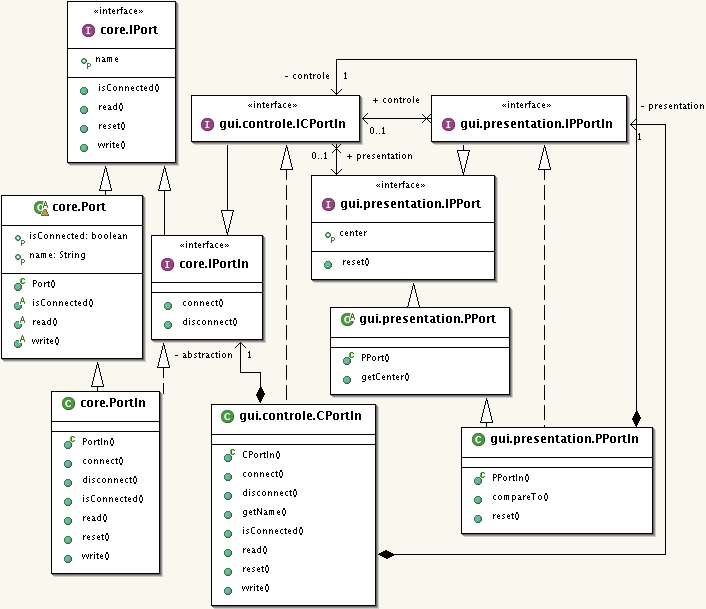
\includegraphics[width=\textwidth]{img/pac/pac_portIn.jpg}
\caption{Composant PAC PortIn}
\end{figure}
\newpage

\subsubsection{Composant PAC PortOut}
\begin{figure}[h!] 
\centering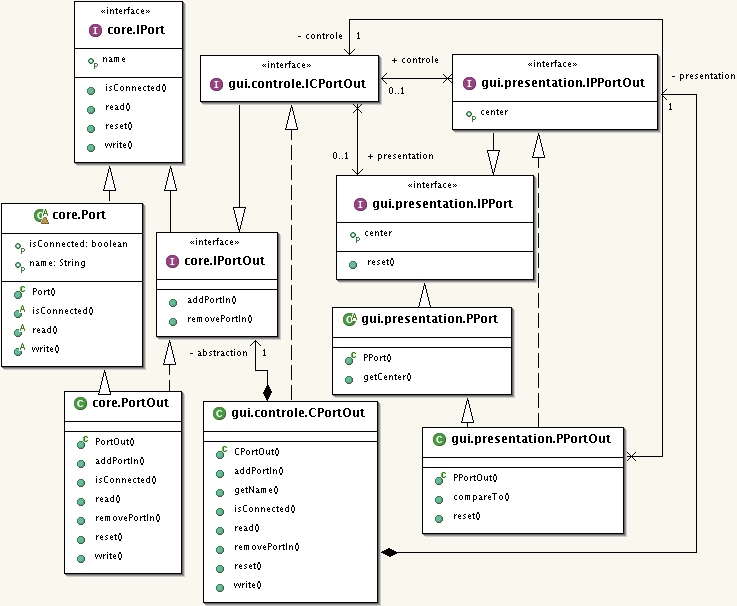
\includegraphics[width=\textwidth]{img/pac/pac_portOut.jpg}
\caption{Composant PAC PortOut}
\end{figure}
\newpage

\section{Interface Graphique}
\subsection{G�n�ralit�s sur l'interface graphique}
\label{interface}
\index{Interface graphique}

Le logiciel s'utilise en grande partie avec la souris. L'interface est donc 
tr�s anim�e pour l'utilisateur. La fen�tre principale de l'interface graphique 
se d�coupe en 3 zones :
\begin{itemize}
\item Une barre d'outils sup�rieure \index{Barre d'outils!superieure@sup�rieure}
\item Un espace de travail \index{Espace de travail}
\item Une barre d'outils inf�rieure \index{Barre d'outils!inferieure@inf�rieure}
\end{itemize}

\begin{figure}[!h]
	\begin{center} 
		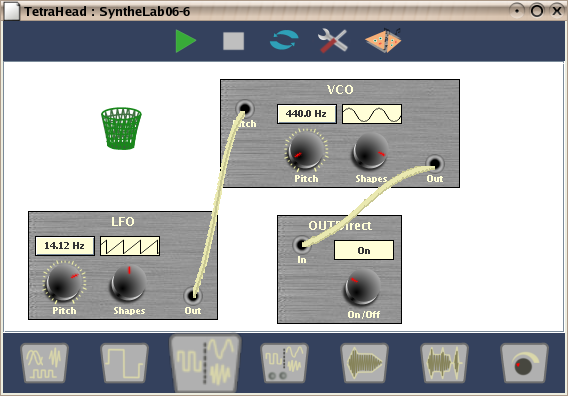
\includegraphics[width=0.7\textwidth]{img/interface/screenshot.png}
		\caption{Capture d'�cran de l'interface graphique}
		\label{connector-ai}
	\end{center}
\end{figure}

La barre sup�rieure contient les boutons qui modifient l'�tat du synth�tiseur 
apr�s un clic de souris : lecture, arr�t, ouverture d'une bo�te de 
dialogue\dots \medskip

La barre inf�rieure contient les boutons qui permettent � l'utilisateur de 
cr�er des modules. Pour cr�er un module, il faut effectuer un drag sur le 
bouton corespondant � ce module. Quand la souris entre dans l'espace de travail, le module y 
est aussit�t ajout�. L'utilisateur peut alors le placer o� il souhaite. \medskip

Pour connecter deux modules, il faut �galement r�aliser un drag'n'drop 
\index{Drag'n'Drop} depuis un port de sortie vers un port d'entr�e. Le nombre 
de connecteurs reli�s � un port de sortie est illimit�. Mais il ne peut y avoir 
qu'un seul connecteur reli� � un port d'entr�e. Quand un utilisateur tire un 
connecteur vers un port d'entr�e, le port d'entr�e se couvre d'une bordure 
rouge quand le curseur est au dessus de lui si ce port est d�j� connect�. 
Si le port d'entr�e est libre et peut donc accepter la connexion, la bordure est verte. \medskip

\begin{figure}[!htpb]
	\begin{center} 
		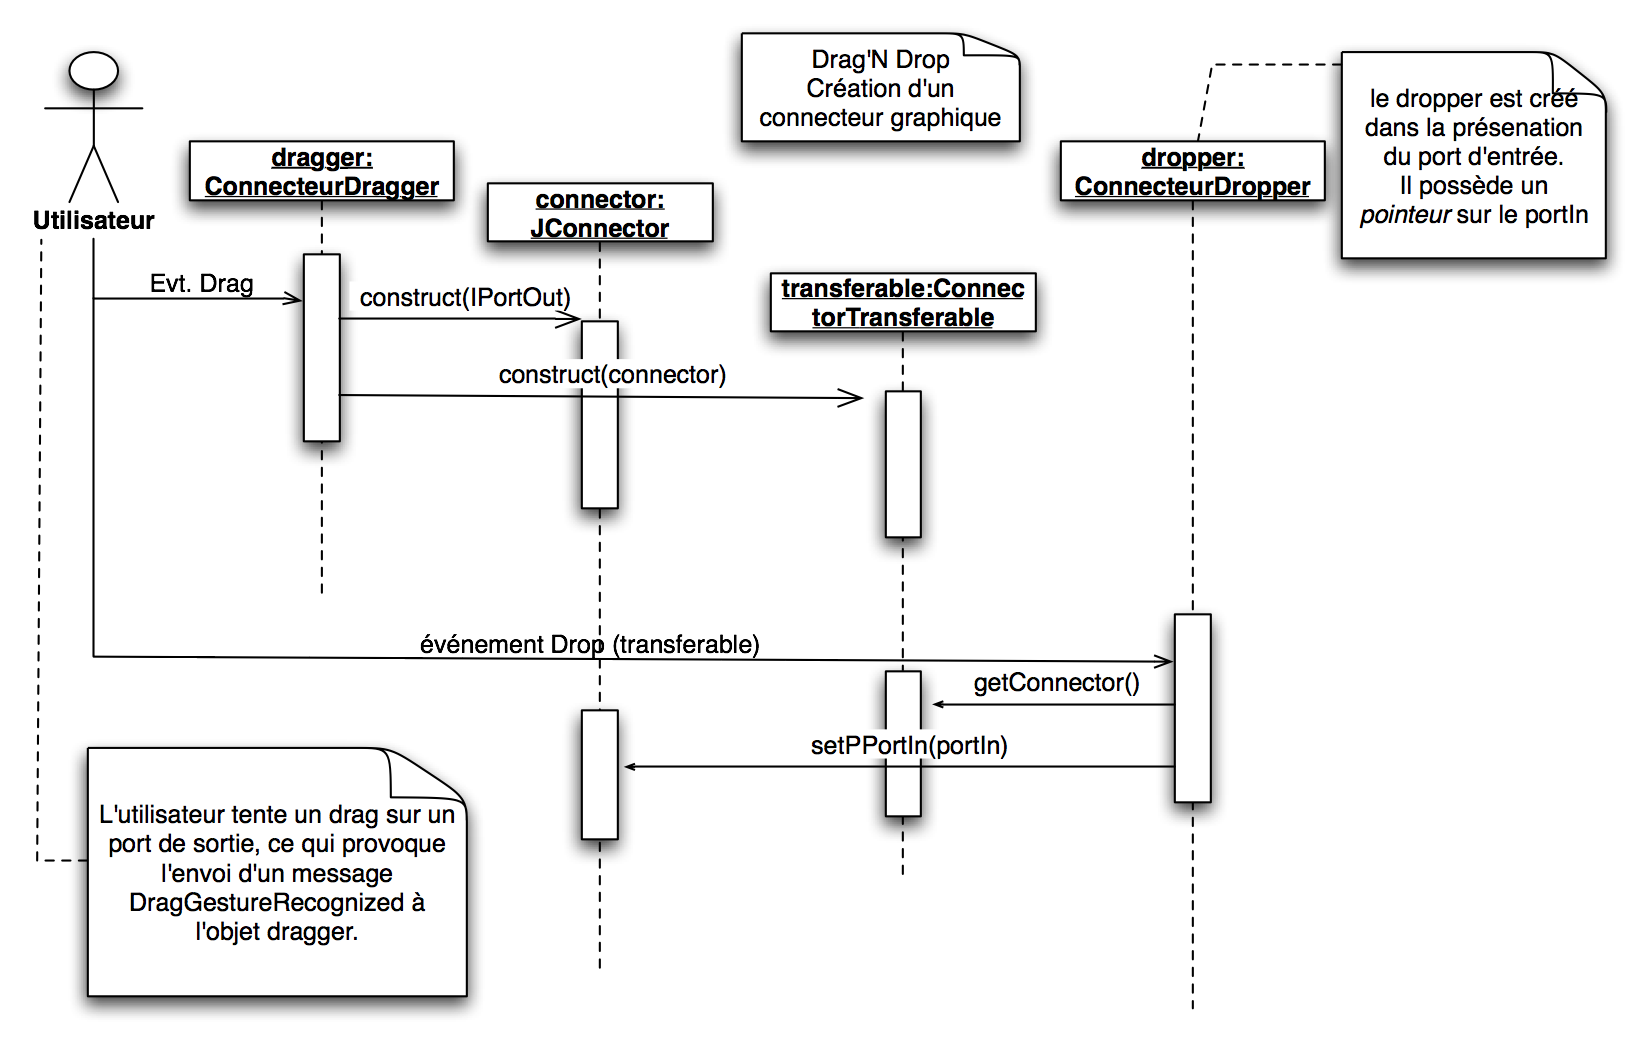
\includegraphics[width=\textwidth]{img/interface/connector-drag-sequence.png}
		\caption{Diagramme de s�quence de la cr�ation du connecteur avec 
		le drag'n'drop AWT}
	\end{center}
\end{figure}

Le changement de valeur des param�tres des modules se fait �galement avec la 
souris. Tous les param�tres, qu'ils soient de types discrets ou continus, sont 
repr�sent�s par un bouton circulaire. La diff�rence visuelle entre les deux est 
que le param�tre continu est entour� de petites graduations. Pour faire varier 
un param�tre discret\index{parametre@Param�tre!discret@discret}, un clic droit 
sur le bouton le fait tourner d'un cran vers la droite et r�ciproquement avec 
le bouton gauche. \medskip

Pour le param�tre continu\index{parametre@Param�tre!continu}, il faut faire 
tourner la souris autour du centre du bouton pendant un clic pour faire varier 
la valeur du param�tre. Une �tiquette situ�e au dessus du bouton indique la 
valeur du param�tre. De plus, pour un param�tre continu, cette �tiquette est 
�ditable afin de pouvoir entrer une valeur au clavier. En effet, en n'utilisant 
que la souris, il est difficile, voire impossible, d'obtenir une valeur 
pr�cise.\medskip

Pour supprimer un connecteur entre deux modules, il suffit de cliquer dessus 
avec le bouton droit. \medskip

Pour supprimer un module, il faut que celui-ci ne soit connect� avec aucun 
autre module. Dans l'espace de travail, se trouve une petite corbeille 
\index{Corbeille}verte. En d�pla�ant un module au dessus de la corbeille, 
celui-ci est supprim�. Au cours du d�placement d'un module, quand le curseur 
passe au dessus de la corbeille, le module dispara�t temporairement. Mais la 
suppression ne s'effectue que si l'utilisateur relache le bouton de la souris 
au dessus de la corbeille. Le module r�appara�t au moment o� la souris quitte 
la corbeille. \medskip

\index{retoaction semantique@R�troaction s�mantique}
La r�troaction s�mantique est assur�e par :
\begin{itemize}
  \item de nombreuses bulles d'aide,
  \item des changements de curseurs de la souris (exemple : pendant un 
  drag'n'drop),
  \item des changements de couleurs (par exemple : pour savoir si on peut 
  connecter deux modules),
  \item des �tiquettes indiquant la valeur des param�tres,
  \item des messages d'erreurs si l'utilisateur essaie une op�ration interdite,
  \item les boutons qui s'agrandissent quand la souris passe dessus\dots
\end{itemize}

\subsection{Package \code{gui}}
\index{Package!gui@\code{gui}}

Ce package regroupe des classes instanciant les diff�rentes fen�tres de 
l'application. \newpage

\subsection{Package \code{gui.connector}}
\index{Package!gui.connector@\code{gui.connector}}

Le package \code{gui.connector} (figure \ref{connector-ai}) contient les 
classes g�rant le connecteur\index{Connecteur} entre deux modules. Le 
connecteur, instance de \code{JConnector} est repr�sent� par une courbe de 
B�zier \index{Courbe de Bezier@Courbe de B�zier} 
\index{Bezier@B�zier|see{Courbe de B�zier}}dont les points de contr�les 
\index{Points de controle@Points de contr�le}sont des instances de 
\code{ControlPoint}. Les classes \code{ConnectorDragger}, 
\code{ConnectorDropper} et \code{ConnectorTransferable} g�rent le drag'n'drop 
AWT. \bigskip

\begin{figure}[!h]
	\begin{center} 
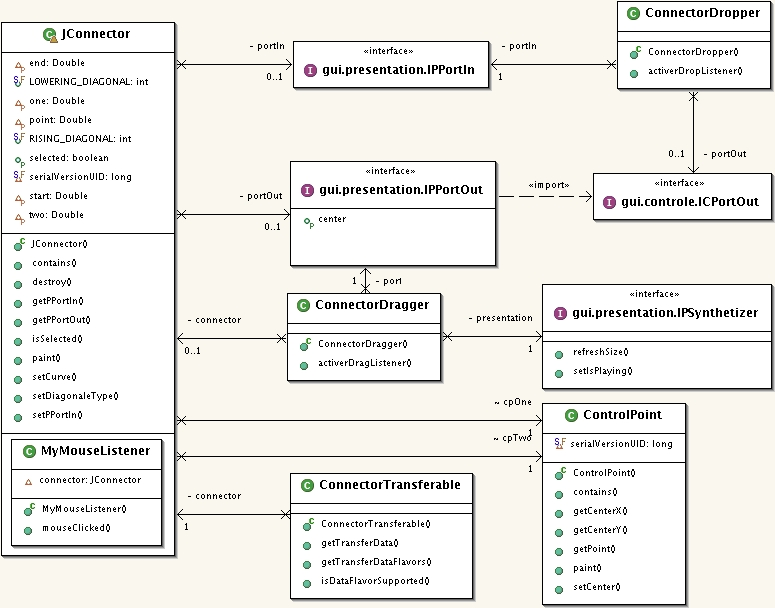
\includegraphics[width=\textwidth]{img/interface/connector-ai.png}
		\caption{Diagramme de classes du package \code{gui.connector}}
		\label{connector-ai}
	\end{center}
\end{figure}
\newpage

\subsection{Packages \code{gui.controle} et \code{gui.presentation}}
\index{Package!gui.controle@\code{gui.controle}}
\index{Package!gui.presentation@\code{gui.presentation}}

Ces packages regroupent les composants \emph{contr�le} et \emph{pr�sentation} 
du mod�le PAC (cf.~section~\ref{pac}, page~\pageref{pac}).

\subsection{Package \code{gui.presentation.parameterAction}}
\index{Package!gui.presentation.parameterAction@\code{gui.presentation.parameterAction}}

Ce package regroupe toutes les classes g�rant le comportement des param�tres, 
discrets et continus, des modules.

\begin{figure}[!h]
	\begin{center} 
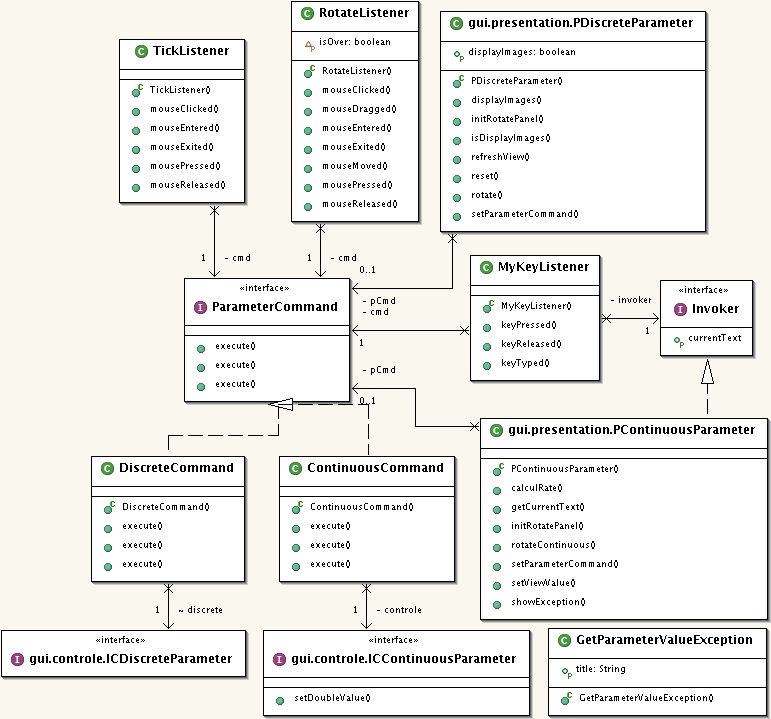
\includegraphics[width=\textwidth]{img/interface/gui-presentation-parameterAction.png}
		\caption{Diagramme de classes du package \code{gui.presentation.parameterAction}}
		\label{toolbar-ai}
	\end{center}
\end{figure}
\newpage

\subsection{Package \code{gui.toolbar}}
\index{Package!gui.toolbar@\code{gui.toolbar}}

\begin{figure}[!h]
	\begin{center} 
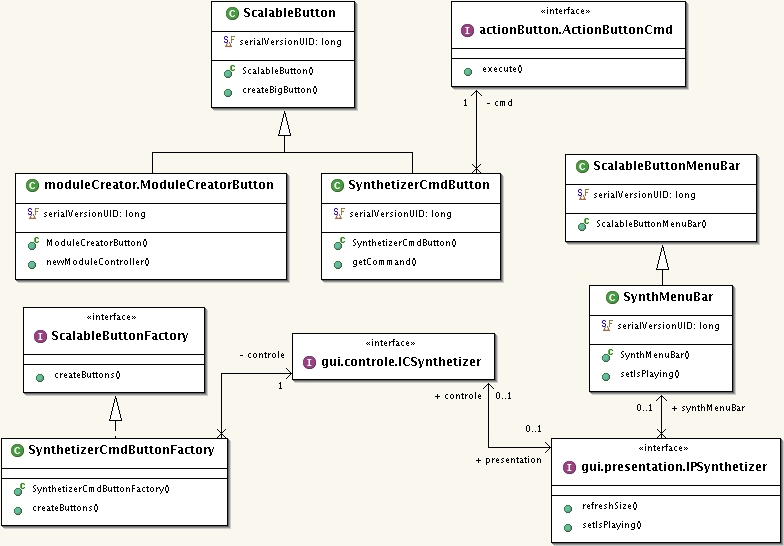
\includegraphics[width=\textwidth]{img/interface/toolbar-ai.png}
		\caption{Diagramme de classes du package \code{gui.toolbar}}
		\label{toolbar-ai}
	\end{center}
\end{figure}

Les classes li�es aux barres d'outils\index{Barre d'outils} sont regroup�es au 
sein du package \code{gui.toolbar}. Les deux barres d'outils sont des instances 
de \code{ScalableButtonMenuBar}. Le constructeur de cette classe prend en 
param�tre un objet \code{ScalableButtonFactory}. Cet objet est une usine charg� 
de produire des boutons. Les boutons g�n�r�s sont ainsi ajout�s dans la barre 
d'outils. L'usine permet la r�utilisation de cette la classe 
\code{ScalableButtonMenuBar}. Les boutons sont des instances de 
\code{ScalableButton} dont le comportement est de s'agrandir quand la souris 
passe dessus. \bigskip

\begin{figure}[!htpb]
	\begin{center} 
		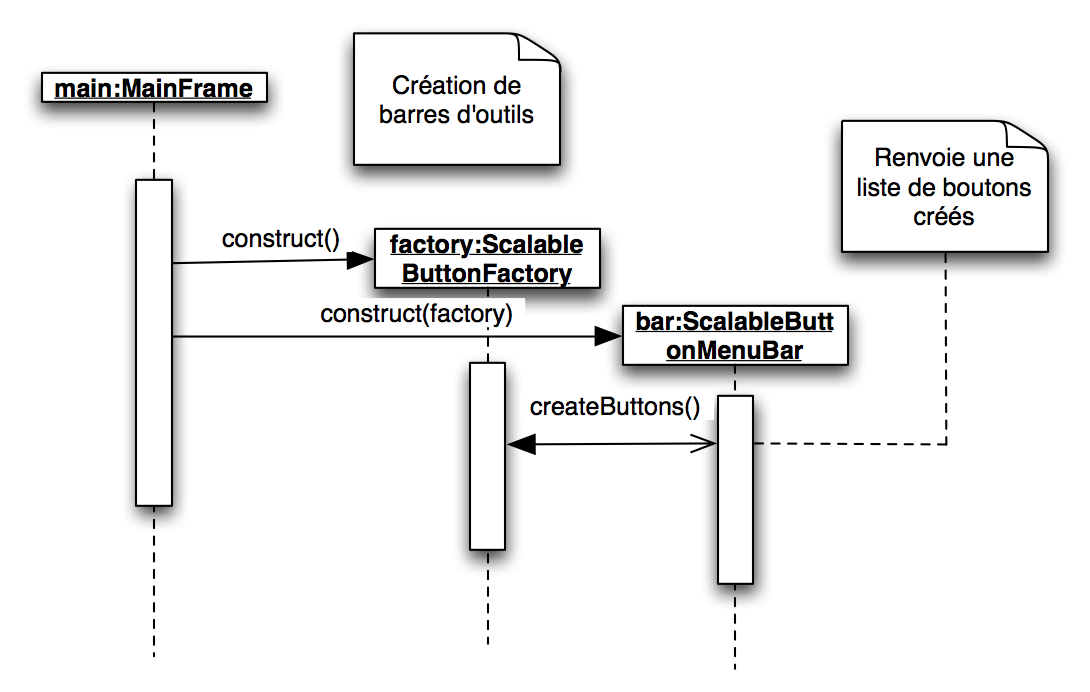
\includegraphics[width=\textwidth]{img/interface/factory-sequence.png}
		\caption{Diagramme de s�quence de cr�ation d'une barre d'outils avec une usine}
	\end{center}
\end{figure}

\index{Package!gui.toolbar.actionButton@\code{gui.toolbar.actionButton}}
\index{Package!gui.toolbar.moduleCreator@\code{gui.toolbar.moduleCreator}}
Ce package contient deux sous-packages : \code{gui.toolbar.actionButton} 
(figure~\ref{actionButton-ai}) et \\
 \code{gui.toolbar.moduleCreator} 
(figure~\ref{moduleCreator}). Chaque package contient des classes param�trant 
la commande des objets \code{ScalableButton}. Le premier sous-package contient 
les commandes de la barre d'outils sup�rieure (lecture, arr�t, reset, options). 
Le second sous-package contient les commandes de cr�ation de modules. \newpage

\begin{figure}[!h]
	\begin{center} 
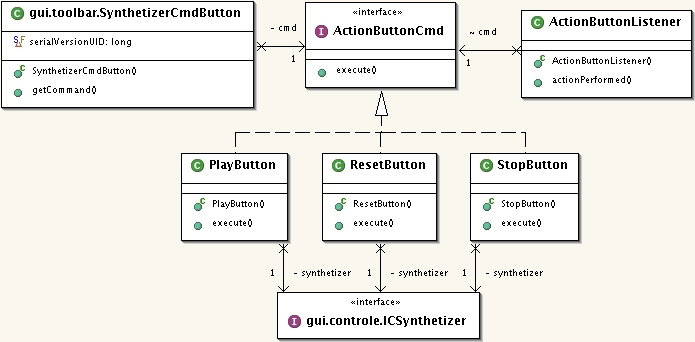
\includegraphics[width=\textwidth]{img/interface/actionButton-ai.png}
		\caption{Diagramme de classes du package \code{gui.toolbar.actionButton}}
		\label{actionButton-ai}
	\end{center}
\end{figure}

\begin{figure}[!h]
	\begin{center} 
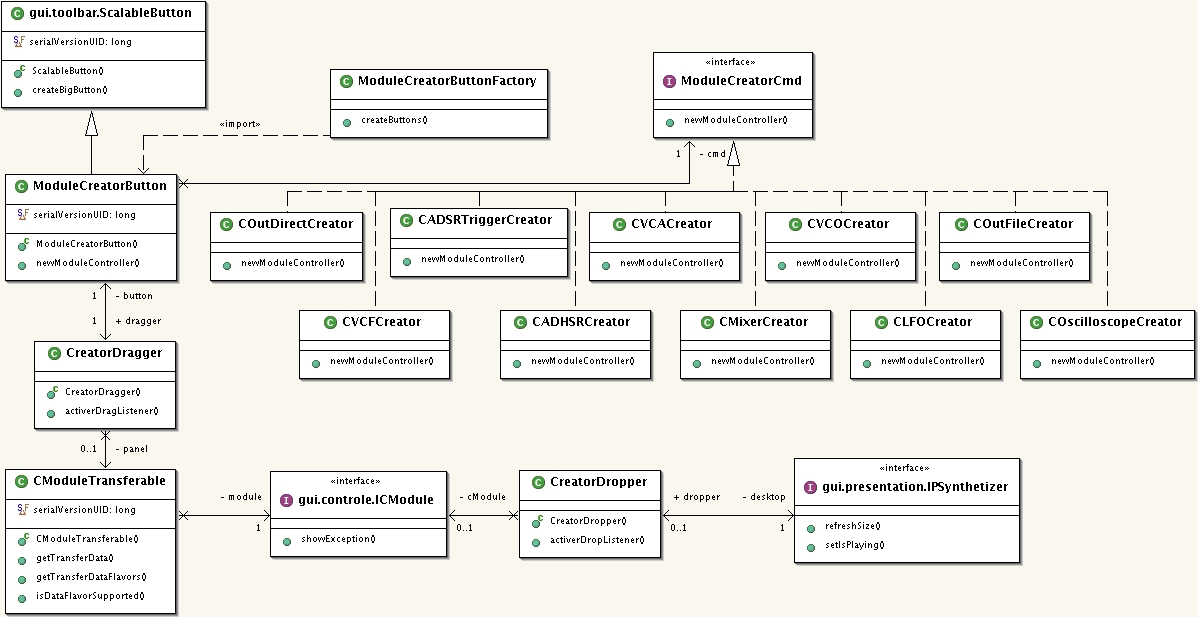
\includegraphics[width=\textwidth]{img/interface/gui-toolbar-moduleCreator.png}
		\caption{Diagramme de classes du package \code{gui.toolbar.moduleCreator}}
		\label{moduleCreator}
	\end{center}
\end{figure}


\section{Archive du projet}


\newpage

\bibliographystyle{plain}
\bibliography{conception}
\newpage

\printindex


% Fin du document
\end{document}
